\documentclass{article}

\usepackage{coursenotes}

\set{AuthorName}{TC Fraser}
\set{Email}{tcfraser@tcfraser.com}
\set{Website}{www.tcfraser.com}
\set{ClassName}{Cosmology}
\set{School}{University of Waterloo}
\set{CourseCode}{Phys 475}
\set{InstructorName}{Niayesh Afshrodi}
\set{Term}{Fall 2016}
\set{Version}{1.0}

\draftprofile[TC Fraser]{TC}{Purple}
\pgfplotsset{
    standardplot/.style={
        axis x line=middle,
        axis y line=middle,
        enlarge x limits=0.05,
        enlarge y limits=0.05,
        every axis x label/.style={at={(current axis.right of origin)},anchor=north east},
        every axis y label/.style={at={(current axis.above origin)},anchor=north east},
        ytick=\empty,
        xtick=\empty,
        width=3in,
        height=2.5in,
        axis line style=thick,
    }
}

\begin{document}

\titlePage

\tableOfContents

\disclaimer

\section{Introduction}


\subsection{History of Cosmology}

The first lecture consisted of everyone introducing themselves and then a brief summary of historical cosmology from Copernicus, to Kepler, Newton, and Einstein. The Copernican principle demonstrated that the earth is not special; Kepler's Laws revealed that the motion of the planets can be described by mathematical tools; Newton's laws unified physical properties observed on earth to those observed in the night sky. Finally, Einstein's equivalence principle further illuminated the equivalence between different observers. All of these observations and discovers have progressed us to the understanding we have today. The \textit{Cosmological Principle} is as follows,

\begin{center}
    \textit{At large scales the universe is homogeneous and isotropic.}\\
    \textit{Equivalently, all observers see the same thing.}
\end{center}

However, there are two important caveats. First, the Cosmological Principle holds on very large scales (typically $\SI{6e22}{\m}$). Second, the Cosmological Principle holds for space but \textit{not} time. This latter caveat was not fully accepted until after Einstein. Einstein was under the motivation that the Universe was static and unchanging because of his unification of space and time (i.e. the homogeneity of space \textit{should} imply the homogeneity of time). However there was an observation that disagrees with this idea. \textbf{Olbers' Paradox} concerns itself with the issue of the darkness of the night sky. If the universe is homogeneous and isotropic, then in every direction one can look in the night sky, there should be a star at some distance away. In dual statement: no point in the night sky should be dark; hence the paradox. The resolution to Olbers' paradox is that the universe must not be infinite. \\

More rigorously, let the solid angle of an object a distance $r$ away with radius $R$ be $\pi R^2 / r^2$. Therefore the total solid angle for all stars should be,
\[ \sum_{i} \f{\pi R_{i}^2}{r_{i}^2} = n_* \intl_{0}^{r\tsb{max}} {4 \pi r^2 \dif r \f{\pi R_{*}^2}{r^2}} \propto r\tsb{max} R_{*}^2 \to \inf \]

In 1922, Hubble discovered the cosmic expansion of the universe which in turn implies the \textit{Big Bang}; following the ``linear'' expansion \textit{backward} in time, then at some point everything needs to be allocated at a singular point. \\

\textit{Remark:} In general, there does not seem to be a clear distinction between cosmology and astrophysics. For clarity, we will consider cosmology to be the evolution of the universe as a \textit{whole}. Of course there will be many exceptions to this focus, when we temporarily divert our attention to high energy particle physics, general relativity and other areas of physics. \\

\subsection{Studying the Universe as a Whole}

To study the paradigm of Cosmology, we will have to study the stuff that composes it. We can learn about the universe as a whole in many ways. For example, most of our observations are via the electromagnetic spectrum ($\ga$/X-ray, UV, optical, IR, $\mu$-waves, radio). Moreover we have the ability to probe the universe through neutrinos, cosmic rays and more recently (due to the work of the LIGO observatory), gravitational waves. \\

\subsubsection{Optical}
The building blocks of the visible/optical universe are:
\begin{itemize}
    \item Stars
    \begin{itemize}
        \item Mass: $M \approx M_{\astrosun} \approx \SI{2e30}{\kg}$
        \item Distance: $D \gtrsim \SI{}{\pc} \approx \SI{3}{\lyr} \approx \SI{3e16}{\m} \approx \SI{2e5}{\AU} $
    \end{itemize}
    \item Galaxies
    \begin{itemize}
        \item Number of stars: $N \approx \SI{1e11}{}$
        \item Mass: $M \approx N \cdot M_{\astrosun}$
        \item Radius: $R \approx \SI{100}{\kilo\pc}$
    \end{itemize}
    \item Globular Clusters
    \begin{itemize}
        \item Number of stars: $N \approx \SI{1e8}{}$
    \end{itemize}
\end{itemize}

Of course, the Milky Way (the galaxy we live in) is observable in the visible spectrum with the naked eye. The Milky Way is a relatively flat disk but appears to us as a thin band due to our location inside it. The approximate thickness of the Milky Way is $\SI{300}{\pc}$ and our distance to the center is roughly $\SI{8.5}{\kilo\pc}$. The central (roughly spherical) bulge in the center of the Milky Way is on the order of $\SI{1}{\kilo\pc}-\SI{2}{\kilo\pc}$. The orbital velocity of the solar system in the Milky Way is $v \approx \SI{220}{\km\per\s}$. The total orbital period is then,
\[ t = \f{2\pi r}{v} \approx \SI{2e8}{\yr} \]
While the age of the universe is $t\tsb{univ} \approx \SI{1.4e12}{\yr}$. \\

Moreover, there are other galaxies in the Universe other than the Milky Way; the most famous one being the Andromeda Galaxy (M31). The `M' stands for Messier. In the 20th century, people started making measurements of the distance to the nearest galaxies (which at the time were unknown objects) and discovered they were much farther than previously thought $d \gtrsim \SI{770}{\kilo\pc}$. \\

Galaxies come in two distinct types: some are elliptical and some are disks (spirals). To characterize a given galaxy, it depends on the size of the central bulge. Disk galaxies (bluer, older) are very ordered and have collated orbits while elliptical galaxies (reder, younger) are almost entirely bulges. \\

A collection of galaxies can form larger structures themselves. The Andromeda and Milky Way galaxies themselves are members of a larger structure known as the \textbf{Local Group} bound together by gravity. Other members of the local group include the Large Magellanic Cloud and various small satellites to the Milky Way. A galaxy group typically has on the order of a few dozens of large objects. \\

Continuing to larger and larger scales, galaxies can form clusters. Some examples include the Virgo cluster, or the Coma Cluster. A galaxy cluster typically has roughly thousands of members and has galaxy speeds $v\tsb{gal} \approx \SI{1000}{\km \per \s}$. Galaxy clusters are the largest known bound structures in the universe with a size on the order of $\SI{1}{\mega\pc}$. \\

Even larger, there are super clusters or voids. These objects are large regions where there are very many galaxies or very few galaxies and are on the order of $d \approx \SI{10}{\mega\pc}$. At larger scales, the universe is homogeneous. The approximate deviation in density is on the order of $n\tsb{gal} \approx \br{4-5} \times \ba{n\tsb{gal}}$. There is an assortment of names for these objects including:
\begin{itemize}
    \item Filaments
    \item Fingers of God
    \item Great wall
    \item Matchstick man
\end{itemize}

\subsubsection{Other Wavelengths}

Looking at the Universe in other wavelengths ($\ga$/X-ray, UV, IR, $\mu$-waves, radio) allows one to view features that are not visible in the optical spectrum. To see the universe in shorter wavelengths like $\ga$/X-ray, UV, we have had to build telescopes outside the earth's atmosphere. Although many things can be learned from making observations in each spectrum, the $\mu$-waves spectrum is of particular importance to cosmology. \\

\begin{center}
    \includegraphics[width=.6\textwidth]{figures/Planck_CMB.jpg}
\end{center}

The \textbf{Cosmic Microwave Background (CMB)} was first discovered by Penzias \& Wilson in 1965 by accident. If the universe is expanding, then at some point in the past hot media would have emitted radiation and cooled to much lower temperatures. The CMB is a isotropic source of radiation that is at a temperature,
\[ T\tsb{CMB} = \SI{2.725 \pm 0.001}{\K} \]
Which was first measured in 1992 by COBE-FIRAS. Recall the blackbody spectrum,
\begin{center}
\begin{tikzpicture}
        \begin{axis}[
            standardplot,
            xmin=0, xmax=10, ymin=0, ymax=2,
            xlabel={$f$},
            ylabel={$\ep_f$},
        ]
        \addplot[domain=0.001:10,smooth,thick, variable=\x,red]  plot ({\x},{\x^3/(e^(\x) - 1)});
        \end{axis}
\end{tikzpicture}
\end{center}

Where $\ep_f$ is the energy of radiation per unit volume per frequency,
\[ \f{\dif E}{ \dif V \dif f} = \ep_f = \f{8\pi h f^3}{c^3\bs{e^{hf/kT} - 1}} \]
Which under appropriate normalization matches the CMB extremely well; making it our most accurate indication for big-bang cosmology. However, there are slight anisotropies in the CMB. The variation in temperature of the CMB is extremely small (discovered COBE-DMR 1992),
\[ \f{\de T}{T} \approx \SI{1e-5}{} \]
For these discoveries, John Marher and G. Smoot shared the Nobel prize in 2006. Since these observations the WMAP (2001) and Planck (2013) projects have obtained higher and higher resolution images of the CMB. \\

In addition to $\mu$-waves, the infrared (IR) spectrum is also important for cosmology. Dust absorbs more and more light at higher and higher frequencies. As such, lower wavelengths are important to be able to see through cosmic dust. As a quick summary, here are some infrared surveys,
\begin{itemize}
    \item 2MASS ($2\mu$, neat IR) stars
    \item IRAS (80's) ($>20\mu$, far IR) dust
    \item Spitzer (new)
\end{itemize}

Moreover X-rays are much more energetic than optical light rays,
\[ E\tsb{optical} \approx \SI{}{\eV} \approx \SI{1.6e-19}{\J} \qquad E\tsb{X} \approx \SI{}{\kilo\eV} \]
The typical temperature of an X-ray is $T\tsb{X} \approx \SI{1e7}{\K}$ which is great for studying clusters of galaxies because most of a clusters mass is in plasma and $T\tsb{plasma} \approx T\tsb{X}$. Clusters are excellent cosmic labs because they are so dense. In fact, our first evidence for dark matter came from studying galaxy clusters via X-rays. \\

Radiowaves are also useful for cosmology because the transition of an electron in a neutral hydrogen atom from spin up to spin down emits weak energy emissions around $\SI{21}{\cm}$. The precision of radiowaves allows one to measure speeds of cosmic bodies by examining shifts in the $\SI{21}{\cm}$ spectrum. The CHIME project is an up-and-coming radiowave telescope.

\subsubsection{Matter in The Universe}

Most of the matter in the universe is made up of particles (with the potential notable exception of dark matter). In truth, the modern perspective on matter is an emergent phenomena of quantum \textit{fields}. From Einstein, we have that,
\[ E^2 = p^2 c^2 + m^2 c^4 \]
Where $E$ is the energy of the particle, $p$ is the momentum and $m$ is the rest mass. If $p \ll m c$ we can take the non-relativistic limit $v = \f{p}{m} \ll c$,
\[ E = \sqrt{p^2 c^2 + m^2 c^4} = mc^2 + \f{1}{2}\f{p^2}{m} + \mathcal{O}\br{m c^2 \f{p^4}{m^4 c^4}} \]
Clearly $\f{1}{2}\f{p^2}{m}$ refers to the standard classical kinetic energy. Higher order corrections to these formulas typically are on the order of $\mathcal{O}\br{c^{-2}}$. On the other hand, for relativistic particles we have that $E \approx pc$ when $v \approx c$. To retain generality, we define the velocity of a particle to be,
\[ \ve{v} = \f{\ve{p}c^2}{E} \]
Here is a breakdown of the contents of the universe: \\
\textbf{Cosmic Content:}
\begin{itemize}
    \item $\%4$ -- baryons/leptons (protons $m\tsb{p} c^2 \approx \SI{}{\giga\eV}$ and electrons $m\tsb{e} c^2 \approx \SI{0.5}{\mega\eV}$)
    \item $\%0.004$ -- radiation (photons $m_{\ga}c^2 = 0$ and neutrinos $m_{\nu}c^2 \approx \SI{0.1}{\eV}$)
    \item $\%25$ -- dark matter (clumpy)
    \item $\%70$ -- dark energy (smooth)
\end{itemize}
The main interactions in the universe are due to photons scattering off of free electrons (\term{Thomas Scattering}) and also weakly interacting neutrinos. We have relative densities,
\[ \rho_{\ga} \approx \rho_{\nu} \approx 10^{-3} \rho_{b} \]
\[ n_{\ga} \approx n_{\nu} \approx 10^{9} n_{b} \]


\subsection{Hubble Law}

The Hubble law (discovered by Hubble) shows that nebulae at further and further distances are moving \textit{away} from us faster and faster. Hubble measured distances (using variable stars) and velocities of spiral nebulae using their Doppler shift (galaxies) using and obtained the following result:
\begin{center}
    \includegraphics{figures/hubble.jpg}
\end{center}
More recent measurements are depicted below:
\begin{center}
    \includegraphics[width=0.7\textwidth]{figures/Modern_Hubble.jpg}
\end{center}
\[ v_{r} = H r \]
Where $r$ is the distance to the object, $v_{r}$ is the radial velocity of that object and $H$ is a constant known as \term{Hubble's Constant}. Hubble's constant has numerical value,
\[ H = 100 \cdot h \SI{}{\km \per \s \per \mega\pc} \]
Where is a dimensionless number measured to an accuracy $h = \SI{0.68\pm0.02}{}$.
To measure velocities, Hubble used the Doppler shift,
\[ 1+ z = \f{\la\tsb{obs}}{\la\tsb{emit}} = \f{1 + \f{v}{c}}{1 - \f{v}{c}} \]
Where $z$ is called the \term{Redshift} and $v$ is the radial velocity of the object.\footnote{In fact, in a homogeneous universe, the only motion is radial.} As a first order approximation in small $v$,
\[ 1 + z = 1 + \f{v}{c} + \mathcal{O}\bs{\br{\f{v}{c}}^2} \]
In the other limiting case, as $v \to c$, we have that ${\la\tsb{obs}}/{\la\tsb{emit}} \to \inf$ which makes $z \to \inf$.\\

To characterize deviations from Hubble's law, we define the peculiar velocity to be,
\[ \ve{v}_p = \ve{v} - H \ve{r} \]
Where it is typical to have $\ba{v_p^2}^{1/2} \approx \SI{400}{\km\per\s}$. Hubble's law was one of the first indications for the Big-Bang. It fact the time since the big bang is approximately,
\[ t\tsb{big bang} = \f{1}{H} \approx \SI{14}{\giga\yr} \]
Hubble's law gives us a picture of the kinematics of the universe.

\section{Newtonian Cosmology}

Now that we have a rough idea of the contents and kinematics of our universe, we shall start to study the dynamics of the universe. In doing so, we will approach an obstacle; as we look at farther and farther objects, Hubble's law dictates that these objects are moving faster and faster. At some point these objects are moving \textit{faster} than the speed of light. As such, in order to do justice to Cosmology, one should study it through the lens of general relativity.\\

Despite this, we can take a shortcut ($\Phi_N = - {GM}/{r}$).
\[ \abs{\Phi_{N}}, v^2 \ll c^2 \quad \text{vs.}\quad \abs{\Phi_{N}}, v^2 \approx c^2 \]
To study local properties of the universe, it is sufficient to use Newtonian physics. Of course, global properties require a relativistic treatment. As such we will first focus on Newtonian Cosmology.\\

Consider two spherical\footnote{Objects that are not spherical exhibit deviations from \cref{eq:next_grav} known as \term{tidal forces}.} masses $M$ and $m$ and the force between them,
\[ F = \f{G M m}{r^2} \eq \label{eq:next_grav} \]
As well as the potential energy,
\[ V = m \Phi_N = -\f{GMm}{r} \]
Another thing of note is that masses are always positive $m \geq 0$. To contrast Newton, the most important equation in Cosmology is the \term{Friedmann equation}. If the universe is homogeneous we can pick a generic point to be the origin for the universe and define a ball of radius $r$ (growing at rate $\dot{r}$) around this point enclosing a mass $M = \f43 \pi r^3 \rho$. By conservation of energy,
\begin{align*}
U &= T + V = \text{const.} \\
&= \f{1}{2} m \dot{r}^2 - \f{GMm}{r} \\
&= \f{1}{2} m \dot{r}^2 - \f43 \pi \rho G m r^2 \eq \label{eq:conser_fried_eq}
\end{align*}
Next define a \term{co-moving} coordinate $\ve{x}$ such that $\ve{r}\br{\ve{x}, t} = a\br{t} \ve{x}$. For each particle at $\ve{x}$, as the universe expands, $\ve{x}$ follows the location of the particle. The physical coordinate of the particle is $\ve{r}$ and the relevant dimensionless scale factor is $a\br{t}$. These concepts hold for all ``origins'' provided that the universe is homogeneous and isotropic. Substituting the co-moving coordinate into \cref{eq:conser_fried_eq} yields the Friedmann equation,
\[ \br{\f{\dot{a}}{a}}^2 = \f{8 \pi G}{3} \rho_b - \f{k c^2}{a^2} \eq \label{eq:friedmann_equation} \]
Where $k$ is defined such that,
\[ k c^2 = - \f{2 U\br{x}}{m x^2} \]
In order for the universe to remain homogeneous, it must be that $k$ does not depend on $x$. Therefore $k$ is a constant in a homogeneous universe. By dimensional analysis on \cref{eq:friedmann_equation} it can be seen that $k$ has dimensions $\text{length}^{-2}$. In general relativity $k$ becomes the curvature of the space. Intuitively, a homogeneous universe has the same curvature everywhere. \\

One misconception associated with the expansion of the universe is that \textit{everything} in the universe is expanding. However, object that are close enough can be bound together by interactions in various fields. As such, the expansion of the universe has little to no observable affect on local objects like planets or people or galaxies. \\

\subsection{Solving the Friedmann Equation}

Solving the Friedmann equation corresponds to solving \cref{eq:friedmann_equation} together with the \term{fluid equation}. The fluid equation comes from the first law of thermodynamics ($\dif E + p \dif V = T \dif S = 0$), which translates to,
\[ E = \pi a^3 x^3 \rho c^2 \qquad V = \f43 \pi a^3 x^3 \]
Which gives the continuity equation,
\[ \dot{\rho} - \f{3\dot{a}}{a} \br{\rho + \f{P}{c^2}} = 0 \eq \label{eq:fluid}\]
Where the pressure $P\br{\rho}$ is determined by the equation of state. Combining \cref{eq:fluid} and \cref{eq:friedmann_equation} gives,
\[ \f{\ddot{a}}{a} = - \f{4 \pi G}{3} \br{\rho + \f{3P}{c^2}} \]
Which is a relativistic manifestation of Newton's law. The difference being the term term involving pressure $P$.

\section{Geometry}

In Euclidean geometry, parallel lines do not intersect and the sum of the interior angles of a triangle sum to $180^o$. However, Euclidean geometry is only a special case:

\begin{center}
\begin{tabular}{|c|c|}
    \hline
    Geometry & k \\
    \hline
    Hyperbolic & -1 \\
    Flat & 0 \\
    Geometry & +1 \\
    \hline
\end{tabular}
\end{center}

\[ \ell = \begin{cases}
    \phi R \sin\br{\f{r}{R}} & k = +1 \\
    \phi r & k = 0 \\
    \phi R \sinh\br{\f{r}{R}} & k = -1 \\
\end{cases} \]
Introduce the spacial components of the \term{Friedmann Robertson Walker (FRW) metric},
\[ \dif s^2 = a^2\br{t}\br{\f{\dif r^2}{1 - kr^2} + r^2 \br{\dif \theta^2 + \sin^2 \theta \dif \phi^2}} \eq \label{eq:FLRW}\]
There is a choice in dimensionality among the terms involved. Typically, $a\br{t}$ is taken to be a dimensionless quantity such that $r$ and $k$ have units. In doing so, we can make the scaling choice of,
\[ a\br{t\tsb{now}} = a\br{t_0} = a_0 \defined 1 \]
Where $t_0$ is used to denote the present time. Therefore $r$ has units of length and $k$ necessarily has units of $\text{length}^{-2}$. Considering the different possibilities for $k$ ($\bc{k < 0, k = 0, k > 0}$), observational data has not been able to distinguish the curvature $k$ of our universe. Experiments suggest it is close to zero. \\

Recall that for an isotropic expansion, we need $a\br{t}$ on the ``outside'' of \cref{eq:FLRW} and so $r,\theta,\phi$ (or $x,y,z$ in flat space) are commoving coordinates. We will also see that galaxies have $r, \theta, \phi$ approximately fixed (in a homogeneous universe).\\

\textit{What is the velocity of a galaxy?} Obviously velocity is the derivative of a distance. However there are many different distances to consider in cosmology. One option is to define the distance between two objects at a fixed time called \term{proper time}. To calculate proper time take $\dif s^2$ at fixed time $t$ and integrating over $\dif r$ and setting $r=0$ to be the reference galaxy. Integrating along a radial line $\dif \phi = \dif \theta = 0$. Thus,
\[ d\tsb{prop} = a\br{t} \underbrace{\intl_{0}^{r} \f{\dif r'^2}{\sqrt{1 - k r'^2}}}_{\chi} \]
Note that for a galaxy, if $r$ is constant then $\chi$ is constant as well.
The \term{proper velocity} in this case is of course,
\[ \dot d\tsb{prop} = \dot a \chi = \dot a \f{d\tsb{prop}}{d} = \br{\f{\dot a}{a}} d\tsb{prop} \]
Which is identical to Hubble's law,
\[ \bc{\dot r = H_0 r} \sim \bc{\dot d\tsb{prop} = \br{\f{\dot a}{a}} d\tsb{prop}}  \]
Therefore it could be that Hubble's constant is a function of time,
\[ H\br{t} = \f{\dot a}{a} \eq \label{eq:hubble_scale_factor} \]
\subsection{Summary of General Relativity}
Without delving into the rigor and formalism of General Relativity, we summarize some of the ideas behind the foundations of GR.\\

The \term{equivalence principle} is best introduced via an analogy to electrostatics. In electrostatics, the force between two charges $Q, q$ is,
\[ F = \f{1}{4\pi\ep_0}\f{Qq}{r^2} \]
Therefore the acceleration on the smaller charge $q$ with mass $m$ is,
\[ a = \f{Qq}{4\pi\ep_0mr^2} = \f{Q}{4\pi\ep_0r^2}\br{\f{q}{m}} \]
Quite characteristically, the acceleration depends on the ratio $q/m$. Therefore an electron and proton will have a very different acceleration when nearby the same charge $Q$. In contrast, gravity behaves \textit{differently}. In gravity,
\[ F = \f{GMm}{r^2} = ma \]
Therefore,
\[ a = \f{GM}{r^2} \br{\f{m}{m}} = \f{GM}{r^2} \]
Therefore any object (regardless of its mass) has the same acceleration; hinting at the fact that gravity is \textit{special}. The equivalence of $m\tsb{grav}$ and $m\tsb{inert}$ then suggests the famous elevator thought experiment. Because of the mass equivalence, no experiment can distinguish the difference between an experiment on earth (in a uniform gravitational field) and a uniform acceleration (like in a rocket). Therefore, if the light from a laser in a rocket appears to bend downward in a rocket (due to the acceleration) it must also be the case that light bends downward toward earth! The resolution between this thought experiment and Fermat's optical principle is that space itself is bending in a gravitational field. The light in a gravitational field follows ``straight'' \term{geodesics}. Freely-falling objects (particles, photons) follow geodesics in space-time. \\

There is an important caveat to the equivalence principle. If the rocketships (elevators) has size comparable to the size of the earth, then the body will experience forces in different directions across its extent in a gravitational field but \textit{not} when uniformly accelerating. These forces are known as \term{tidal forces}. So in Gr space time must behave like special relativity on small scales. In SR the spacetime line element is written as,
\[ \dif s^2 = - c^2 \dif t^2 + \dif x^2 + \dif y^2 + \dif z^2 \]
Photons taking at speed $c$ has the defining property that,
\[ \dif s^2_\ga  = 0 \eq \label{eq:null_geodesics}\]
Which can be stated as: \textit{photons travel on null geodesics}. Therefore the \term{full FRW metric} must be,
\[ \dif s^2 = - c^2 \dif t^2 + a^2\br{t}\br{\f{\dif r^2}{1 - kr^2}} + r^2 \br{\dif \theta^2 + \sin^2 \theta \dif \phi^2} \eq \label{eq:FRW_full}\]
To solve for the equations of motion or geodesics of photons, one simply needs to solve \cref{eq:FRW_full} under the constraint that \cref{eq:null_geodesics}. In summary the following comparison holds,
\begin{center}
\begin{tabular}{|l|l|}
    \hline
    Special Relativity & General Relativity \\
    \hline
    Special observers are inertial & Freely falling \\
    Light follows null geodesics & same \\
    Particles move in straight lines & Particles follow geodesics \\
    Empty universe / No curvature & Not empty universe / Curvature \\
    \hline
\end{tabular}
\end{center}
Note that the ``flat'' universe $(k=0)$ is spatially flat, but curved in space-time. \\

In summary, general relativity is composed of a Lorentzian space-time,
\[ \De s^2 = - \br{c \De t}^2 + \De x^2 + \De y^2 + \De z^2\]
And the notion that gravity is consequence of the curvature of space-time. The particulars of how matter and curvature are harmonious is embodied in Einstein's Equations. As a high level summary, Einstein's equations dictate the following relationship.

\[ \text{curvature} = \br{\f{8\pi G}{c^2}} \cdot \text{energy-momentum-pressure density} \]

\subsection{Einstein's Equations and Cosmology}

In cosmology (and under the cosmological principle), there is a unique solution to Einstein's equations. It is the FRW metric previously derived above in \cref{eq:FRW_full}
\[ \De s^2 = - c^2 \De t^2 + a^2\br{t}\br{\f{\De r^2}{1 - kr^2}} + r^2 \br{\De \theta^2 + \sin^2 \theta \De \phi^2} \]
Where $k$ determines the geometry of the spacial parts of the universe,

\begin{center}
\begin{tabular}{|c|c|c|}
    \hline
    k & Geometry & Boundary \\
    \hline
    -1 & Hyperbolic & Open \\
    0  & Flat & Open \\
    +1 & Geometry & Closed \\
    \hline
\end{tabular}
\end{center}

As far as we can tell, $k\approx 0$. Another possibility is that the universe has a non-trivial topology; albeit no observable evidence suggests this.

The Einstein equation relates functions of the metric $(\dif s^2 = \cdots)$ to the energy content of the universe. Typically, the Einstein equations are $10$ non-linear equations. When applied to a homogeneous universe (as is considered in cosmology), the Einstein equations reduce to $2$ equations. One of which is the Friedmann equation,
\[ \br{\f{\dot a}{a}}^2 + \f{k c^2}{a^2} = \f{8 \pi G}{3} \rho \]
Where $kc^3/a^2$ is related to the energy content but here it is related to the curvature as well (same $k$ as in FRW metric).

\subsection{Review}
As a review we have the following set of cosmological equations.
The Friedmann equation:
\[ H^2 + \f{k}{a^2} = \f{8\pi G}{3} \rho \eq \label{eq:review_friedmann}\]
Where the Hubble parameter is,
\[ H = \f{\dot a}{a} \]
The Fluid equation:
\[ \dot \rho + 3 H \br{\rho + p} = 0 \eq \label{eq:review_fluid} \]
Combining \cref{eq:review_friedmann,eq:review_fluid} we arrive at,
\[ \f{\ddot a}{a} = - \f{4 \pi G}{3}\br{\rho + \f{3P}{c^2}} \]

\section{Redshift \& Expansion}
So far we have looked at Doppler shift as a source for redshift. Of course redshift is also caused by an expanding universe. At small velocities we have,
\[ \f{\De \la}{\la} = \f{v}{c} = \f{H \De r}{c} \]
Where $\De r$ is a physical local distance $\De r = c \De t$,
\[ \f{\De \la}{\la} = \f{\dot a \De t}{a} = \f{\De a}{a} \]
Integration gives us that,
\[ \la \propto a \]
Intuitively, the length of waves in the universe scales with the size of the universe.
\[ 1 + z = \f{\la\tsb{obs}}{\la\tsb{emit}} = \f{a\br{t\tsb{obs}}}{a\br{t\tsb{emit}}}  \]
Where $t\tsb{obs}$ is typically taken to be today. The quantity is $z$ is known as redshift. As an example, the farthest galaxy that we can see has a redshift of approximately $z \approx 7-8$. In contrast, the redshift of the cosmic microwave background is at $z \approx 1100$.

\section{Equations of State}
All ``materials'' in the universe have different equations of state $P\br{\rho}$. Matter or dust has effectively a pressure of zero ($P = 0$). This is because the actual pressure is much less that the characteristic pressure of $\rho c^2$, meaning we can omit it from the fluid equation,
\[ \dot\rho = \f{3 \dot a}{a} \br{\rho + \f{P}{c^2}} \approx \f{3 \dot a}{a} \br{\rho} \]
Therefore for dust and matter,
\[ \f{\dot \rho}{\rho} = 3\f{\dot a}{a} \implies \rho = \f{\rho_a}{a^3} \]
Plugging this into the Friedmann equation gives us that,
\[ \dot a^2 = \f{8\pi G \rho_a}{3a} \implies a = \br{\f{t}{t_0}}^{2/3} \]
By convention, we take $t_0$ to be today and $a\br{t_0} = 1$ when making observations. We have that $1 + z = \f{1}{a}$. Therefore in a matter dominated universe, $a$ scales as $t^{2/3}$. Therefore Hubble's parameter scales as,
\[ H = \f{\dot a}{a} = \f{2}{3t} \]
However for radiation, we have that $P = \f{1}{3} \rho c^2$ (this holds for photons and neutrinos). A similar analysis yields the relationship,
\[ \rho = \f{\rho_a}{a^4} \]
Plugging into the Friedmann equation once again gives,
\[ \dot a^2 = \f{8\pi G \rho_a}{3a} \implies a = \br{\f{t}{t_0}}^{1/2} \]
Which indicates that $H = 1/2t$. \\

Additionally, we can incorporate dark energy (cosmological constant fluid) to obtain,
\[ P = - \rho c^2 \implies \rho = \rho_{*} \implies a = e^{Ht}\]
Our discovery of the acceleration of the expansion of the universe indicates that there is a dark energy contribution to the expansion of the universe. Depending on the composition of the universe, there are different behaviors for the expansion of the universe. Initially, (when $a$ is smaller) radiation is dominating. Latter matter will dominate and then finally dark energy.
\begin{center}
    \begin{tikzpicture}
        \draw[->] (0,0) -- (0,3) node[above]{$\rho \propto H^2$};
        \draw[->] (0,0) -- (4,0) node[right]{$a$};
        \draw [cyan] plot [smooth, tension=0.7] coordinates { (0.1,2.7) (1,1.6) (3.1,0.7)};
        \draw [cyan] (3.1,0.7) -- (4,0.7);
        \draw [cyan] (0.7, 2.4) node[]{$\f{1}{a^4}$};
        \draw [] (1, -0.2) node[below]{$\f{1}{3000}$}--  (1, 0);
        \draw [cyan] (2, 1.5) node[]{$\f{1}{a^3}$};
        \draw [cyan] (3.7, 1.1) node[]{$\text{const.}$};
    \end{tikzpicture}
\end{center}
The number density of particles scales as,
\[ n = \f{n_0}{a^3} \]
While the number density or energy density of photons is given by,
\[ E_{\ga} = \f{hc}{\la} \propto \f{1}{a} \]
Looking at the Friedmann equation we have that,
\[ \underbrace{\f{1}{2} \dot a^2}_{\text{K.E.}} - \underbrace{\f{4 \pi G}{3} \rho a^2}_{\text{P.E.}} = -\f{k}{2} = E\tsb{tot} \]
\section{Making Measurements}
It is very remarkable (and somewhat bizarre) that we can describe the large scale structure of the universe. This is a unique feature of cosmology. \\

The question remains, how exactly are we able to measure cosmological features. As an examine, we measure Hubble's constant $H_{0}$ by using redshift $z$ and distance $r$.
\[ z = \f{v}{c} = \f{H_0 r}{c} \implies H_0 = \f{zc}{r} \]
Measuring Hubble's constant is as old as cosmology itself. Nonetheless, there are a few subtleties associated with measuring $H_0$. As it turns out, it is very each to measure the redshift $z$ by comparing the spectrum of distance bodies to those in the laboratory. Additionally, Hubble's law is not exact.
\[ z = \f{H_0 r}{c} \pm \de z = \f{H_0 r}{c} \pm \f{v\tsb{pec}}{c} \]
Where $v\tsb{pec}$ are peculiar velocities that dominate at small distances. Typical peculiar velocities are roughly $v\tsb{pec} \approx \SI{600}{\km \per \s}$. Measuring an accurate Hubble's constant $H_0$ requires making measurements on very large scales. \\

The harder part of measuring Hubble's constant is the measurement of distances $r$; there is no perfect way of measuring distance. Typically, distances are measured using parallaxes of distance bodies. In the past Hipparcos was the main survey of parallaxes of distance bodies. More recently, the GAIA telescope was launched. \\

A better technique for measuring distances is to make use of \term{standard candles}.
\[ F = \f{L_s}{4 \pi r^2} \]
Where the luminosity $L_s$ can be determined based on some standard process or model and the flux $F$ is easily measured with instruments near earth. The best standard candles that are used today are variable Cepheids stars and type 1a supernovae. We say that these processes are standardizable. All of these methods of measuring distance form a cosmic distance ladder that can be used to perform calibrations and consistency checks.\\

\begin{center}
    \includegraphics[width=0.7\textwidth]{figures/cosmic_ladder.jpg}
\end{center}

Our most precise measurements today are as follows.
\begin{center}
\begin{tabular}{|c|c|c|}
    \hline
    Method & $H_0$ & Source\\
    \hline
    Supernovae & $\SI{73.24 \pm 1.74}{\km \per s}$ & Riess \textit{et al.} 2016\\
    CMB & $\SI{66.93 \pm 0.62}{\km \per s}$ & Planck 2015\\
    \hline
\end{tabular}
\end{center}
Evidently there is some tension associated with these measurements, namely that it is possible that supernovae are not as standardizable as most scientists assume. It is also possible that there is new physics that we do not understand yet.\\

As was mentioned previously, some works define $h$ such that,
\[ H = \SI{100}{\km \per \s \per \mega\pc} \cdot h \]

Again recalling the Friedmann equation (\cref{eq:friedmann_equation}),
\[ H^2 = \f{8 \pi G}{3}\rho - \f{k}{a^2} \]
We can define the \term{critical density} $\rho_{c}\br{t}$ to be,
\[ \rho_{c}\br{t} = \f{3 H^2\br{t}}{8 \pi G} \]
To be the density if $\rho = \rho_c$. Cosmologists define \term{density parameters},
\[ \Om_i \br{t} = \f{\rho_i\br{t}}{\rho_c\br{t}} \]
Where $i$ can be any material in the universe (radiation, matter, dark energy). The density parameters sum to,
\[ \Om\tsb{tot} = \sum_{i} \Om_i = 1 + \f{k}{a^2 H^2} \]
Which can be used to measure the value of $k$. If $\Om\tsb{tot}$ is $1$, then it must be that $k = 0$. Today we obtain,
\begin{align*}
    \rho_c\br{t_0}
    &= \SI{1.88e-26}{\kg \per \m^3} \cdot h^2\\
    &= \SI{2.78}{} \cdot h^{-1} \cdot \f{\SI{1e11}{} M_{\astrosun}}{\br{h^{-1} \SI{}{\mega\pc}}^3}
\end{align*}
Each of these density parameters is a function of time $\Om_i = \Om_i\br{t}$. We define for today,
\[ \Om_{i0} = \Om_i\br{t_0} \]
Some authors defined $\Om_k$ such that,
\[ \Om_k = \f{-k}{a^2 H^2} \implies \Om\tsb{tot} + \Om_k = 1 \]
Where observations today indicate,
\[ \abs{\Om_k} \lesssim 0.01 \eq \label{eq:k_om} \]
\section{Densities}
Consider a flat spacetime that has expanded since the bigbang.

\begin{center}
    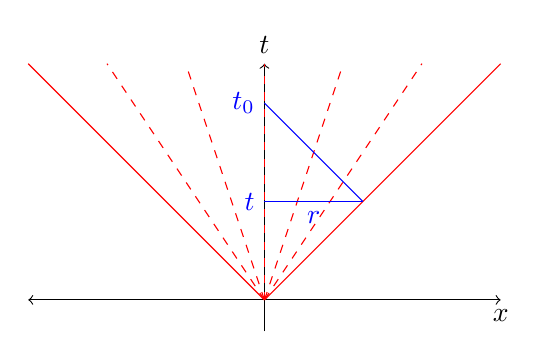
\begin{tikzpicture}
        \coordinate (t0) at (0, 2.5);
        \draw[<->] (-3, 0) -- (3, 0) node[below]{$x$};
        \draw[->] (0, -0.4) -- (0, 3) node[above]{$t$};
        \draw[red] (0, 0) -- (3, 3);
        \draw[red, dashed] (0, 0) -- (2, 3);
        \draw[red, dashed] (0, 0) -- (1, 3);
        \draw[red, dashed] (0, 0) -- (0, 3);
        \draw[red, dashed] (0, 0) -- (-1, 3);
        \draw[red, dashed] (0, 0) -- (-2, 3);
        \draw[red] (0, 0) -- (-3, 3);
        \draw[blue] (t0) node[left]{$t_0$} -- (1.25, 1.25);
        \draw[blue] (0, 1.25) node[left]{$t$} -- node[below]{$r$} (1.25, 1.25);
    \end{tikzpicture}
\end{center}

Due to the geometry of this universe ($r$ is not a co-moving distance),
\[ c\br{t_0 - t} = r \qquad v = \f{r}{t} \]
Therefore,
\[ c\br{t_0 - \f{r}{v}} = r \]
Which gives,
\[ v = \f{r}{t_0 - \f{r}{c}} \implies \f{c}{v} = \f{ct_0}{r} - 1 \]
Therefore the redshift can be computed,
\[ 1 + z = \sqrt{\f{1 + \f{v}{c}}{1 - \f{v}{c}}} = \sqrt{\f{ct_0 / c}{-2+ct_0/r}} = \br{1 - \f{2r}{ct_0}}^{-1/2} \approx 1 + \f{r}{ct_0} + \f{3}{8}\f{4 r^2 }{c^2t_0^2} \]
We define the \term{deceleration parameter} $q$,
\[ q = -\f{\ddot a}{aH^2} = -\f{\ddot a a}{\dot a^2} = \f{\Om_m}{2} + \Om_r - \Om_{\La} \]
The deceleration parameter acts as a sub-leading correction to the expansion of the universe. When it was observed that experimentally $q < 0$, one have to conclude that $\Om_{\La} > \f{\Om_m}{2} + \Om_r$. In fact in 1999 (Nobel Prize in 2011) dark energy was discovered with value,
\[ \Om_{\La} \approx \SI{0.7}{} \]
Combining these observations with measurements from the CMB (namely \cref{eq:k_om}), one obtains the density of matter in the universe,
\[ \Om_{m} \approx 0.3  \]
With decomposition,
\[ \Om\tsb{DM} + \Om\tsb{Baryon} = \Om_{m} \qquad \Om\tsb{DM} \approx 0.26 \qquad \Om\tsb{Baryon} \approx 0.04 \]
The main distinction between dark matter and dark energy is that dark matter is pressure-less but dark energy has an measurable negative pressure. \\

\textit{What the Heck is $\La$?} Einstein's equations are as follows,
\[ \La g_{\mu \nu} + G_{\mu \nu} = \f{8 \pi G}{c^2} T_{\mu \nu } \eq \label{eq:eins_eqn}\]
Where $G_{\mu \nu}$ encodes the curvature, $g_{\mu \nu}$ is the metric and $T_{\mu\nu}$ is the energy-momentum tensor. Einstein first introduced the cosmological constant $\La$ in order to enforce a static universe. Nonetheless, today we appreciate it as the source of our dynamic universe. It is also possible to move $\La g_{\mu \nu}$ to the RHS of \cref{eq:eins_eqn} and treat it as a form of matter,
\[ \rho_{\La} = + \f{\La}{8 \pi G} \qquad P_{\La} = - \f{\La c^2}{8 \pi G} \]
Where $P_{\La} = - \rho_{\La} c^2$ and $\Om_{\La} = \f{\La}{3 H^2}$. It is convenient to think of $\La$ as contributions that are due to the vacuum of empty space. Observationally we measure,
\[ \Om_{\La} \approx \SI{0.7}{} \]
Nonetheless in Quantum Mechanics, the predicted contributions due to vacuum fluctuations are,
\[ \Om_{\La} \approx \SI{1e60}{} - \SI{1e120}{} \]
This is known as the \term{cosmological constant problem}. It is important to also understand that,
\[ w_{Q} = - \f{P_Q}{\rho_Q c^2} = \begin{cases}
    -1 & \text{for $\La$}\\
    \SI{-1.01 \pm 0.05}{} & \text{Planck 2015}\\
\end{cases} \]
More accurate measurements of $w_{Q}$ could possibly point to the origin of the cosmological constant problem. Other approaches to fixing the CCP would be to discovering a new theory for gravity.
\subsection{Age of The Universe}
One of the earliest indications of the presence of $\La$ was from measuring the age of the universe. From our current measurement of $H_0$ we have that,
\[ t_H = \f{1}{H_0} = 9.77 h^{-1} \SI{}{\giga \yr} \approx \SI{14}{\giga \yr} \]
However if $\Om_m = 1$,
\[ a \propto t^{2/3} \implies H_0 = \f{2}{3 t_0} \implies t_0 = \f{2}{3}t_H \approx \SI{9.3}{\giga \yr} \]
Which would not have been a problem until measurements on the ages of globular clusters indicated ages of roughly $t \approx \SI{10}{\giga \yr} - \SI{13}{\giga \yr}$.
\section{Geodesics}
So far we have talked about the Friedmann equations and how to solve them for various density contributions. This gives us $a\br{t}$. Alternatively one could measure distances to galaxies to determine how $a\br{t}$ changes with time. Unfortunately, the timescales for doing this accurately are very large. \\

Alternatively, we can make use of the FRW metric,
\[ \dif s^2 = - c^2 \dif t^2 + a^2\br{t} \bs{\f{\dif r^2}{1 - k r^2} + r^2 \dif \te^2 + r^2 \sin^2 \te \dif \phi^2} \]
The distance between two points (say $A,B$) can be obtained by integrating $\dif s$,
\[ \s{S} = \int_A^B \dif s \]
If $\s{S}$ is real, then the distance is space-like and the two locations can not communicate. Alternatively if $\s{S}$ is imaginary then we say that the two locations are time-like separated. Finally, a light ray has null distance.
\begin{center}
\begin{tabular}{|c|c|c|}
    \hline
    $\s{S}$ & Separation & Communication \\
    \hline
    Real & Space-Like & Not Possible \\
    Imaginary & Time-Like & Possible \\
    0 & Null & -- \\
    \hline
\end{tabular}
\end{center}
Geodesics can be found by extremizing $\s{S}$ (i.e. either maximizing or minimizing). In particular, time-like geodesics maximum the time contributions to distance while space-like geodesics minimize $\s{S}$. We define the \term{proper time} of a geodesic to be $\tau$ such that,
\[ -c^2 \dif \tau^2 = \dif s^2 \]
In cosmology we are interested in the light that travels to us from distant galaxies. Let $r=r_g$ be the distance to a distant galaxy.
\begin{center}
\begin{tikzpicture}
    \begin{scope}
        \tikzstyle{every node}=[fill=black, draw=black, circle, thick, text=black, scale=0.3]
        \node (us) at (0,2) {};
        \node (gal) at (2,0) {};
    \end{scope}
    \draw (us) node[above]{$r_0 = 0$};
    \draw (gal) node[below]{$r_{g} = r$};
    \draw[dashed, ->] (gal) -- node[below left]{$\dot \te, \dot \phi = 0$} (us);
\end{tikzpicture}
\end{center}
Since the light ray has no angular deviation ($\dif \te = \dif \phi = 0$), the FRW metric reduces to,
\[ \dif s^2 = - c^2 \dif t^2 + \f{a^2 \dif r^2}{1 - kr^2} \]
Solving this metric gives,
\[ \f{c \dif t}{a\br{t}} = - \f{\dif r}{\sqrt{1 - kr^2}} \]
\[ c\int_{t}^{t_0} \f{\dif t'}{a\br{t'}} = \int_{0}^{r} \f{\dif r'}{\sqrt{1 - kr^2}} = \begin{cases}
    r & k = 0 \\
    \f{1}{\sqrt{k}}\sin^{-1}\br{\sqrt{k}r} & k > 0\\
    \f{1}{\sqrt{-k}}\sinh^{-1}\br{\sqrt{-k}r} & k < 0\\
\end{cases} \]
Solving the time integral is impossible without knowing the behaviour of $a\br{t}$. Recall that for $\La = k = 0$ we have that,
\[ a\br{t} = \br{\f{t}{t_0}}^{2/3} \]
This gives us,
\[ r = c \int_{t}^{t_0} \br{\f{t'}{t_0}}^{-2/3} \dif t' = 3 c t_0 \]
It is important to note that $r$ is not a physical distance. Instead it is just a co-moving coordinate. As such, it should be alarming that $ r / t_0 = 3 c > c $ seems to be faster than the speed of light. \\

\textit{How do we measure distances via flux}?
Consider a detector that aims to measure light coming from a distance galaxy. Let this detector subtend a solid angle of $\dif \Om$. Then the distance to the galaxy can be measured using,
\[ \dif_L^2 = \f{L}{4\pi F} \]
Where $L$ is the luminosity of the object ($\bs{\text{E}}/\bs{\text{T}}$) while $F$ is the observed flux on the detector ($\bs{\text{E}}/\bs{\text{T}}\bs{\text{Area}}$). In flat space $d_L$ corresponds to a regular distance. However in a curved spacetime, this is not generally the case. The flux observed can be directly computed from the number of photons emitted.
\[  F = \f{N_{\ga} E_{0,\ga}}{\De t_0 a_0^2 r^2 \dif \Om} \]
Where as the number of photons emitted can be determined from the luminosity,
\[ N_{\ga} = \f{L \De t}{E_\ga} \f{\dif \Om}{4 \pi} \]
Combining these results yields (and that $\De t_0 / \De t = E_\ga / E_{0, \ga} = 1 + z$),
\[ F = \br{\f{E_{0,\ga}}{E_{\ga}}} \br{\f{\De t}{\De t_0}} \f{L}{4 \pi \br{a_0 r}^2} \]
Therefore $d_L$ in general is,
\[ d_L = a_0 r\br{1 + z} \]
Relating this to the acceleration parameter,
\[ a\br{t} = a_0 + \dot a \br{t-t_0} + \f{1}{2} \ddot a \br{t- t_0}^2\]
\[ q = -\f{a \ddot a}{\dot a^2} \]
Therefore for $k=0$,
\[ r\br{z} = \int\f{c \dif t}{a\br{t}} \]
And thus we recover a Hubble law (with the augmentation of higher order terms),
\[ H_0 d_L = z + \br{\f{1}{2} - q} z^2 + \s{O}\br{z^3} \]
This can be used to measure $\La$,
\[ q = \f{\Om_m}{2} - \Om_\La \]
Alternatively we can measure distances via angular size,
\[ d_A = ar = \f{r}{1+z} \]
There are two ways of measuring distances in cosmology $d_A, d_L$. Fundamentally the luminosity distance and angular distance are related,
\[ \f{d_L}{1 + z} = r = d_{A} \br{1 + z} \]
It is important to note that $d_A$ does not tend to infinity as $z$ tends to infinity. We demonstrate this explicitly for a standard cosmology $k=0$.
\[ H^2 = \f{8 \pi G}{3} \rho =\f{8 \pi G}{3} \br{\f{\rho_{m, 0}}{a^3} + \rho_\La}\]
\[ H_0^2 = \f{8 \pi G}{3} \rho_{c, 0} \]
Together gives,
\[ \f{H^2}{H_0^2} = \Om_{0, m} \br{1+z^3} + \Om_{0, \La} \]
Therefore,
\[  a\br{t}\dif r = c\dif t = c \f{H_0}{\dif t H} = \f{c \dif h_0 a}{H} =- \f{c \dif h \br{1+z}}{H_0 \sqrt{\Om_{0,m} \br{1 + z}^3 + \Om_{0,\La}}} \]
Which implies,
\[ r\br{z} = \f{c}{H_0} \int_{0}^{z} \f{\dif z}{\sqrt{\Om_{0,m} \br{1 + z}^3 + \Om_{0,\La}}} \]
Which is an integral that can be solved numerically quite easily.

\section{Dark Matter}
We have talked about how cosmology behaves with different material components (matter, radiation, dark energy, curvature). For the last century, we have been trying to understand the behaviors of each of these components; dark energy being one of the latest problems to tackle. \\

The universe has turns out to be much simpler than we previously thought; namely that the universe is homogeneous and isotropic on large scales. On the contrary, the universe is far more complicated and exotic than we previously thought. The current matter density in the universe is given by the current critical density,
\[ \rho_{c,0} = \f{3 H_0^2}{8 \pi G} = h^2\times\SI{1.88e-26}{\kg \per \m^3} \quad h \approx 0.7 \]
One of the objectives of cosmologists is to compare this critical density to observed densities in the universe. The first method used to measure the typical mass content of the universe was to look at stars. The main source of energy in stars is nuclear fusion. In the early 1930's this property started to become well understand. Astronomers are able the color, luminosity and temperature in order to determine the mass of a star. The theory of stellar mass and evolution reveals a the mass to luminosity ratio of main sequence stars (to first order) is,
\[ \f{M}{L} \propto \f{M_{\astrosun}}{L_{\astrosun}} \]
In order to measure mass, we measure the flux received from a large cluster or collection of stars. Over a solid angle in the sky $\de \Om$,
\[ \text{Flux} = \br{\f{M}{L}}^{-1} \int \f{\br{\de \Om r^2 \dif r} \rho_{*}}{4 \pi \dif^2_L} \]
Rearranging and rewriting $\rho_{*}$ in terms of $\Om_{*}$ (also let $z \ll 1$),
\[ \text{Flux} = \br{\f{M}{L}}^{-1} \int \f{ \dif r}{1 + z} \Om_{*} \rho_c \]
\[ \text{Flux} = \br{\f{M}{L}}^{-1} r\tsb{max} \Om_{*} \f{3H_0^2}{8 \pi G} \]
By observationally measuring the flux (and using $H_0, r\tsb{max} = cz\tsb{max} / H_0, M/L \propto M_{\astrosun} / L_{\astrosun}$), cosmologists calculate
\[ \Om_{*} = \SI{0.005}{} \]

So the question remains, what is the source of the rest of the mass associated with $\Om_{m} \approx 0.23$?
\subsection{Dark/Faint Baryons}
One possibility is that the rest of the mass is made up of faint baryonic matter that we do not see like intergalactic plasma. This possibly is the leading theory for what is termed the \term{missing baryon problem}. \\

Another possibility is that the remaining mass is made up of brown dwarfs (massive objects that aren't quite large enough to be stars). Brown dwarfs are very faint, but are still slightly luminous. Of the nearby brown dwarfs that we can see, there is not sufficient evidence to suggest that the source of missing mass is brown dwarfs.\\

Another possible is related to Big Bang nucleosynthesis. Most of the elements in the universe are hydrogen and helium; unlike here on earth where there is an assortment of elements. There is a very nice way of explaining the abundance of lighter elements in the universe. The only way that stars get there energy is through nuclear fusion; turning hydrogen into helium. Big Bang nucleosynthesis suggests that the Big Bang is a source for much heavier elements. The Big Bang is so hot that it is feasible to produce heavier elements like Helium, Deterium, and Lithium. In particular there is a seminal paper by Alfa, Betha, and Gammow that demonstrates there would only be enough time to produce small amounts of $\text{H}, \text{He}, \text{D}, \text{Li}$.
\begin{center}
    \begin{tabular}{|c|c|}
        \hline
        Substance & Portion \\
        \hline
        H & $75\%$\\
        He & $25\%$\\
        D & $10^{-5}$\\
        Li & $10^{-7}$\\
        \hline
    \end{tabular}
\end{center}
Comparing these densities with those measured today, we can get an estimate on the rough density of baryons in the universe,
\[ 0.021 \leq \Om_{b}h^2 \leq 0.025 \]
Therefore,
\[ 0.04 \leq \Om_B \leq 0.05 \]
This upper limit demonstrates that $\Om_B$ could \textit{not} be larger than $0.05$ (otherwise there would a different production of heavier elements during the big bang). Therefore, baryons could never explain the discrepancy between $\Om_{*}$ and $\Om_m$. \\

In summary, the usual suspects are not sufficient to explain the missing mass problem.

\subsection{Dynamical Cosmology}

In the 1930's Oort started looking at the dynamics (velocity) of stars in the solar neighborhood and Zwicky began observing the velocities of galaxies in the Virgo cluster of galaxies. By looking at the oscillations of stars about the bulk mass of a cluster of stars, one can measure the bulk mass of the cluster itself. Moreover, measuring the radial velocity (through deviations in the redshift) of galaxies in the Virgo cluster one can determine the velocities relative to the cluster.
\[ v^2 = \f{G M\br{< R}}{R} \]
In the 1960's and 1970's Rubin and others started looking at the rotation curves of spiral galaxies. What they found was the following profile for rotational velocities in galaxies,
\begin{center}
    \begin{tikzpicture}
        \draw[->] (0,0) -- (0,3) node[above]{$v$};
        \draw[->] (0,0) -- (4,0) node[right]{$d$};
        \draw [red] plot [smooth, tension=0.4] coordinates { (0,0) (1,2.2) (3,2.2) (4,2.2)};
    \end{tikzpicture}
\end{center}
The galaxies were rotating much faster than would be allowed by the stellar mass observed. For a time, his results were not taken too seriously.
Oort's results suggested,
\[ \f{M}{L} \approx \br{3-4} \f{M_{\astrosun}}{L_{\astrosun}} \]
Zwicky's results suggest that,
\[ \f{M}{L} \approx 400 \f{M_{\astrosun}}{L_{\astrosun}} \]
While Rubin's results demonstrate that ${M\tsb{tot}}/{M_{*}} > 3$. \\

All of these results are the foundations for believing in the existence of dark matter. Within spiral galaxies, the mass of dark matter to the mass of stars is typically comparable. Albeit at very large scales the measured proportion of dark matter is much much larger. \\

All of these results suggests a very peculiar property of dark matter: dark matter is dissipation-less. Dark matter does not cool and lose energy. Regular matter can cool down and form very dense objects while dark matter cannot. Our current understanding is that dark matter sits in \term{Halos} around galaxies. There is more and more dark matter the further one looks outside a galaxies.

\subsection{Clusters of Galaxies}

The intergalactic plasma between galaxies in a cluster is typically held at,
\[ T \sim \SI{1e7}{\K} - \SI{1e8}{\K} \]
With density $\rho \sim \SI{1e3}{}\rho_c$. In the intergalactic plasma, the mass of baryons is $M_B = 5-10 M_{*}$. Therefore we can write,
\[ \f{\Om_B}{\Om_m} = \f{M_B}{M\tsb{tot}} \]
Which gives us a great way of measuring $\Om_m$. Modeling the intergalactic plasma as a gas in hydrostatic equilibrium we have that,
\[ \f{\dif P\tsb{gas}}{r} = \rho\tsb{gas} \f{GM\br{<r}}{r} \]
Which provides an avenue for measuring $M\br{<r} \approx M\tsb{tot}$.\footnote{The pressure can be determined from X-ray emissions.} The Chandra satellite has measured the relevant components of intergalactic plasma. These results yield the estimate of,
\[ \Om_M \approx 0.4 \]

\subsection{Structure Formation and CMB}

In the early universe, it is believe that there are two components of the universe,
\begin{enumerate}
    \item Dark Matter
    \item Baryons \& Photons
\end{enumerate}
We clump baryons and photons together because they are constantly interacting in the early universe. Since dark matter is very cold, energy does not propagate through dark matter. This is distinct from baryons and photons because they are very hot permitting sound waves to travel. Using the CMB, we can get the most precise measurement of $\Om_M / \Om_B$.
\[ \Om_B = \SI{0.049\pm0.001}{} \qquad \Om_M = \SI{0.315\pm0.017}{} \]
Adding the cosmological contributions $\Om_{\La} \approx 0.7$ predicts,
\[ \Om\tsb{tot} = 1.00 \pm 0.01 \]

Another possibility to explain dark matter is not to consider dark matter as actual matter at all. Although we will not discuss these in this course, but they typically involve modifications to Einstein's general theory of relativity (or in some cases Newton's gravity). Ultimately, we do not know.

\section{Cosmic Microwave Background (CMB)}
The cosmic microwave background represents our best evidence of big bang cosmology to date. Today we understand Hubble's law as a consequence of the cosmological principle. In the past, cosmology hit a fork in interpretation. The homogeneity of space in the universe and Einstein's special relativity (placing space and time on equal footing) should suggest that time is also homogeneous. The desire to make cosmology and special relativity compatible naturally led to the idea of a \term{steady-state cosmology} (Bondi, Gold, \& Hoyle) however the steady-state cosmology ran into problems of energy conservation. The competing theory at a similar time was \term{big bang cosmology} (Gamow \& others). One of the predictions of big bang cosmologists was big bang nucleosynthesis which agrees with measurements on the current baryon densities of the universe. More convincingly, big bang cosmology predicted left-over radiation from the early universe and was discovered by Penzias \& Wilson to be a perfect blackbody with temperature $T = \SI{2.725\pm0.001}{\K}$. The radiation energy density is then,
\[ \ep_{\ga} = \al T\tsb{CMB}^4 = \SI{4.17e-19}{\J\per\m^3} \]
And thus,
\[ \Om_{\ga} = \f{\ep_\ga}{\rho_c c^2} = \SI{5.04e-5}{} \]
Recall that the density of fluids in the universe scale with $a$ as,
\[ \rho_{\ga} \propto \f{1}{a^4} \quad \rho_{m} \propto \f{1}{a^3} \quad\rho_{\La} \propto 1 \quad\rho_{k} \propto \f{1}{a^2} \]
Which means that in the early universe when $a$ was smallest, radiation was dominant. The redshift at which matter and radiation were on equal scales is current $z\tsb{eq} \approx 3400$. For a black body,
\[ \ep\br{f} \dif f \propto \f{f \dif f}{e^{hf /k T} - 1} \]
But $f \propto a^{-1} = 1 + z$ and $T \propto a^{-1}$ and thus $\ep\br{f} \propto a^{-4}$. Therefore we know that the blackbody spectrum for radiation is \textit{not} affected by cosmic redshift. This is a very special property of radiation which enables us to know that the CMB was a blackbody in the early universe because it is a blackbody today.\\

We can also look at the CMB using number densities of photons. The number density of photons is,
\[ n_\ga = \f{\ep_\ga}{3 k T} \approx \SI{3e8}{\m^{-3}} \]
And the number density of baryons,
\[ n_B = \f{\Om_B \rho_c}{m_B} \approx \SI{0.26}{\m^{-3}} \]
Therefore there are nearly 2 billion more photons than baryons.
\[ \f{n_\ga}{n_B} \approx \SI{1.7e9}{} \]
To contrast, there are roughly $\SI{1e31}{}$ particles of matter in a single cubic meter. Although there are many more photons, the majority of energy is in baryons. \\

\subsection{Formation of the CMB}

To figure out how the CMB formed we need to think a little bit about the hydrogen atom. Most of the material we see in the universe today is neutral and in the form of atoms or molecules. At high enough temperatures, this neutral atoms would have been ionized. From quantum mechanics, we know that if the temperature scale is larger that $k T > \SI{13.6}{\eV}$ then the electron of the neutral atom will escape. From the previous section we know that the energy of photons in the universe behaves like,
\[ E_\ga = 3 k T = \f{\SI{7e-4}{\eV}}{a} \]
Which means that $E_\ga = \SI{13.6}{\eV}$ at a scale $a^{-1} = 1+ z = \SI{2e4}{}$. The cross section of a photon is the Thomson cross-section $\si_T = \SI{6.65e-29}{m^2}$ which means the mean-free path for photons is,
\[ \la_\ga = \f{1}{n_e \si_T} \]
From this, we can conclude that the Hubble distance scale for a photon $d_H = \f{c}{H}$ scales as $t$ while the mean free path scales as $t^2$. We have that $\la_\ga \ll d_H$ which means that at the photons scatter many times over the cosmic time scales which means that the universe would be opaque. \\

At low temperatures electrons and protons have low enough energies to form bound atoms. As it turns out, this does not occur at exactly the moment when $E_\ga = \SI{13.6}{\eV}$. Nonetheless when hydrogen atoms are formed at low enough temperatures, the approximate cross section for photons drops because only photons of very specific frequencies can be absorbed by electrons,
\[ \si_R = \si_T \br{\f{E}{\SI{10}{\eV}}}^{4} \eq \label{eq:rayleigh_cross_section}\]
Which is known as the \term{Rayleigh cross section}. When the temperature decreases below the characteristic energy $\SI{10}{\eV}$ photons become approximately transparent and can travel freely. However, interactions between photons and matter are more complicated when $E \ll \SI{10}{\eV}$ and \cref{eq:rayleigh_cross_section} breaks down. \term{Recombination} refers to the time when $\f{n_p}{n_H} = \f{n_e}{n_H} < 0.1$ when all of the free particles combine to form atom, while \term{decoupling} refers to the time in which the scattering of photons off electrons roughly ceases,
\[ \dif t = \f{H \dif t}{H} = \f{\dif h a}{H} = \f{\dif a}{\br{1 + z} H\br{z}} \]
\[ 1 = \int_0^z n_e\br{z} \si_T \br{z} c \dif t = \int_0^z n_\ga\br{z} \si_T \br{z} c \f{\dif a}{\br{1 + z} H\br{z}} \]
This forms the \term{surface of last scattering},
\[ \f{n_\ga}{n_b}e^{-\f{\SI{13.6}{\eV}}{kT}} \sim 1 \implies kT = \f{\SI{13.6}{\eV}}{\rho_m \underbrace{\br{n_\ga / n_B}}_{\SI{1e9}{}}} \sim \SI{0.65}{\eV} = k \cdot \SI{7400}{\K} \]
This is very approximate, order of magnitude guess at this temperature. More accurately we can compute,
\[ T\tsb{rec} \simeq \SI{3600}{\K} \quad T\tsb{dec} \simeq \SI{3000}{\K} \]
\[ z\tsb{dec} \approx \SI{1100}{\K} \quad r\tsb{dec} \approx \SI{14}{\giga\pc} \quad t\tsb{dec} \approx \SI{3.5e5}{\yr} \]
These better estimates come from the \term{Saha Equation}. In thermal equilibrium, the following process is in complete equilibrium,
\begin{center}
    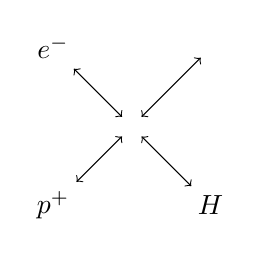
\begin{tikzpicture}
        \draw (-1, 1) node[](e){$e^{-}$};
        \draw (-1, -1) node[](p){$p^{+}$};
        \draw (1, -1) node[](H){$H$};
        \draw (1, 1) node[](ga){$\ga$};
        \draw (0, 0) node[](o){};
        \draw[<->] (e) -- (o);
        \draw[<->] (p) -- (o);
        \draw[<->] (ga) -- (o);
        \draw[<->] (H) -- (o);
    \end{tikzpicture}
\end{center}

\[ N_e = N_p \]
\[ \f{N_e + N_p}{2} + N_H = \text{const.}  \]
\[ \mu_e + \mu_p = \mu_H = \SI{13.6}{\eV} \]
\[ X \defined \f{n_e}{n_B} = \f{n_p}{n_B} \]
\[ \br{1 - X}n_B = n_H \]
Therefore,
\[ \f{1 - X}{X^2} = 3.8 \f{n_B}{n_\ga}\br{\f{kT}{m_B c^2}}^{3/2}  e^{\f{\SI{13.6}{\eV}}{kT}} \]
Setting $X = 0.1$ and solving this equation numerical gives $T \simeq \SI{3600}{\K}$.

\section{Structure Formation in The Universe}

If the universe was \textit{perfectly} homogeneous and isotropic, humans could not exist let alone galaxies and large structures. We do however see stars, star clusters, galaxies, clusters of galaxies and large scale structures. The question remains, how and why does the matter in the universe tend to cluster together.\\

Galaxy redshift surveys are able to map the positions of millions of galaxies. These surveys indicate that the universe appears homogeneous on the largest of scales but the maps also show walls, voids and filaments. In particular we can define the the number density of galaxies at a co-moving distance $r$ to be $n_g\br{r}$ such that,
\[ \ba{n_g\br{r}} = \bar n_g \bs{1 + \xi\br{r}} \]
Where $\xi\br{r}$ is found to be,
\[ \xi\br{r} = \br{\f{r}{\SI{7}{\mega\pc}}}^{-2} \]

\section{Anisotropies}

Structure formation is intimately linked to the formation of structures in the early universe via clustering. The COBE survey discovered anisotropies in the CMB. \\

The temperature deviation $\De T$ at the angular position $\te, \varphi$ in the CMB is given by,
\[ \f{\De T}{T} \br{\te, \varphi} = \f{T\br{\te, \varphi} - \bar T}{\bar T} \]
Where $\bar T$ is the mean temperature of the CMB and $T\br{\te, \varphi}$ is the measured temperature. Expanding $\De T/ T$ in terms of spherical harmonics gives,
\[ \f{\De T}{T} \br{\te, \varphi} = \sum_{\ell = 1}^{\inf} \sum_{m = -\ell}^{\ell} a_{\ell m} Y_{m}^{\ell} \br{\te, \varphi} \]
From this defines the radiation angular power spectrum $C_{\ell} = \ba{\abs{a_{\ell m}}^2}$. Theory is able to predict $C_{\ell}$ while we observe,
\[ \bar C_{\ell} = \f{1}{2\ell + 1} \sum_{m = - \ell}^{\ell} \abs{a_{\ell m}}^2 \]
Where $T_0 = \SI{2.725}{\K}$ is the temperature of the CMB measured today. Theoretical CAMB models of the anisotropies can be plotted against WMAP results. Below, the vertical axis of the following plot is a scaled version of $C_{\ell}$, namely,
\[ \f{1}{2 \pi}T_0^2 \ell \br{\ell + 1} C_{\ell} \]
\begin{center}
    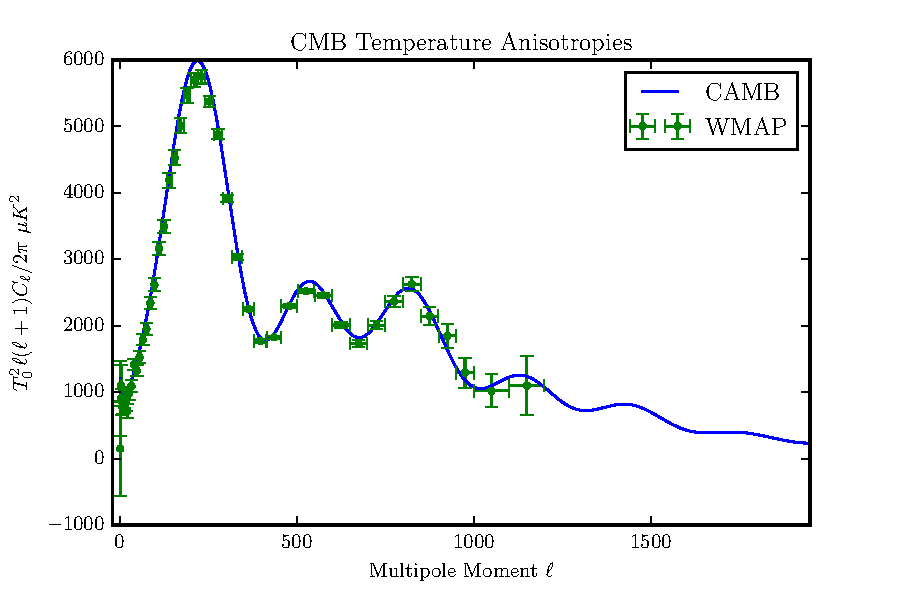
\includegraphics{figures/anisotropies.pdf}
\end{center}
The vertical error bars come from the approximate error reported in the WMAP results. The horizontal error bars are attributed the fact that the multipole values reported by WMAP are binned values. For each bin $\bs{\ell_L, \ell_R}$, the reported $C_{\ell}$ value is an unweighted average of each contribution,
\[ C_{\ell_L}, C_{\ell_{L}+1}, \ldots, C_{\ell_{R}-1}, C_{\ell_{R}}  \]
Qualitatively speaking, the CAMB model and the WMAP measurements share the same features and the error bars are mostly in agreement. \\

Roughly speaking for $\hat n_1 \cdot \hat n_2 = \cos \te$,
\[ \ba{\f{\De T}{T}\br{\hat n_1}\f{\De T}{T}\br{\hat n_2}} \sim \f{\ell \br{\ell + 1}}{2 \pi} C_\ell  \]
The first peak of the anisotropy plots can be related to and thus constrain the values of $\Om_k$ in our universe. The Planck data predicts,
\[ \abs{\Om_k} \leq 0.003 \]

Our best understanding of the origin of structures ($z \geq \SI{e6}{}$) is due to Planck,
\[ \xi\br{r} \simeq \SI{2e-9}{}\br{\f{r}{\SI{20}{\mega \pc}}}^{0.032\pm 0.006} \]


The question remains, why are there fluctuations and what do they accomplish for formation? The gravitational instability of the matter at the surface of last scattering defines a hierarchy. \\

Consider a matter dominated universe,
\[ \Om_m = 1 \qquad \Om_{\La} = 0 \qquad a \propto t^{3/2} \]
If we allow for density deviations $\Om_m = 1 + \ep$ where $0 < \ep \ll 1$ we can define the \term{over density} $\de$ such that,
\[ \de = \f{\de \rho\br{x, t}}{\bar \rho\br{t}} = \f{a\br{t}}{a\br{t_0}} \f{\de \rho\br{x, t_0}}{\bar \rho\br{t_0}} \]
Where typically, $\de \ll 1$. As an exercise, you can show that $\de \propto a$ by considering a spherical region of the universe with $k > 0$ but $\abs{\Om_k} \ll 1$ with $\Om_k = 0$. However, when $\de \sim 1$ you form galaxies and clusters which require numerical simulations. In doing these simulations, it is important to also consider radiation pressure in the early universe and the sound waves they induce.\\

We can also define the idea of \term{bias}. The number density of galaxies should have functional dependence on the matter density in the universe,
\[ n_g\br{x} \simeq f\bs{\rho_m\br{x}} \]
Where $f$ may depend on time. Then,
\[ \de_g = \f{\de n_g}{\bar n_g} = \der{\ln f}{\ln \rho} \cdot \de  \]
Where $b = \der{\ln f}{\ln \rho}$ is the bias. For small galaxies, $b \sim 1$ and for big galaxies and clusters $b \sim 2-3$.


\section{Early Universe}

It is a cosmological triumph that we can describe the entire universe using $6$ free parameters. Early universe cosmological is relatively simple; it is governed by linear equations and is absent of complex structures. This is in contrast to other areas of study like weather or evolutionary biology where the equations are non-linear and messy. The CMB dominates the radiation density of the Universe,
\begin{align*}
    T\tsb{CMB} &= \SI{2.725}{\K}\\
    \Om\tsb{rad} &= \SI{5.0e-5}{}
\end{align*}
In addition to photon contributions, the entire universe was also occupied by neutrinos. Neutrinos we first discovered in the 1930's because neutrinos are only weakly interact with matter. \\

\subsection{Neutrinos}

On small scales, gravity is the weakest force interacting with matter. However, on larger scales, gravity dominates. The strong nuclear force is the strongest force by far on the scale of nuclei. The weak force is the second weakest force, next to gravity. Neutrinos interact though gravity and the weak force. The Higgs boson also interacts through the weak force. As an example, an isolated neutron is unstable and decays via the following process,
\[ n \to p^+ + e^- + \bar \nu \]
Where $p^+$ is a proton, $e^-$ is an electron and $\bar \nu$ is a neutrino. This process has an approximate half-life of $t_{1/2} \sim \SI{10}{\min}$. It is important to note that no other process (outside weak interactions) converts neutrinos to protons. In 1998 we discovered $\nu$'s have mass. Art McDonald won the Nodel Prize in 2015 for this discovery. The interaction cross-section of neutrinos as a function of energy is $\si\br{E} \propto E^2$ which means that neutrinos become less reactive at low temperatures. In the early universe, photons and neutrinos are thought to be in thermal equilibrium. This assumption fixes the temperature of neutrinos.
\[ T_{\nu} = \br{\f{4}{11}}^{1/3} T\tsb{rad} = \SI{1.95}{\K} \]
Where the energy density is,
\[ \Om_{\nu} = 3 \times \f{7}{8} \times \br{\f{4}{11}}^{4/3} \Om\tsb{rad} = \SI{0.68}{}\cdot\Om\tsb{rad} \]
Where the ``$3\times$'' is due to the the fact that neutrinos have three generations or varieties. The ``$7/8$'' is due to the fact that neutrinos are fermions. This tells us that $41\%$ of the energy is due to neutrinos while photons are responsible for the remaining $59\%$.\\

Boson statistics differ from fermion statistics (Bose-Einstein vs. Fermi-Dirac),
\[ \ep_\ga\br{f} \propto \f{f^3 \dif f}{e^{hf/kT} - 1} \quad \ep_\nu\br{f} \propto \f{f^3 \dif f}{e^{hf/kT} + 1} \]
Roughly speaking the number density of neutrinos is,
\[ n_\nu = \f{1}{e^{h f/kT} + 1} \]
Which is always greater than $1$. This is a manifestation of the Pauli-Exclusion principle. \\

Heretofore, we have been treating neutrinos as essentially massless. In reality we have lower bounds on the masses of neutrinos,
\[ m_\nu^1 > \SI{0.05}{\eV} \quad m_\nu^2 > \SI{0.02}{\eV} \quad m_\nu^3 > 0 \]
The reason why we only have lower bounds is because neutrino oscillation experiments can detect the difference in the squares of the masses of neutrinos $\br{m^i}^2 - \br{m^j}^2 \neq 0$. From this knowledge we suspect that at least $2$ $\nu$'s are non-relativistic now. We we ignore the neutrino mass, we calculate the time when radiation and mass densities are equal is,
\[ \f{\Om_r\br{a}}{\Om_m\br{a}} = \f{\Om_\ga + \Om_\nu}{\Om_m} \times \f{1}{a} \implies 1 + z\tsb{eq} = \f{1}{a\tsb{eq}} = \SI{3400}{} \]
This means that $T\tsb{eq} = \f{\SI{2.725}{\K}}{a\tsb{eq}} = \SI{9700}{\K} \approx \SI{1}{\eV}$ which is much larger than the mass of the neutrinos. Therefore neutrinos are relativistic in the this time period.
In order to calculate the time at equality we need to make use of the Friedmann equation,
\[ H^2 = \f{8\pi G}{3}\br{\rho_m + \rho_r + \rho_\La} \]
Doing so is left as an exercise. The time at equality is,
\[ t\tsb{eq} = \SI{5.6e4}{\yr} \]
Compare this to the time of decoupling which occurs slightly after (note that neutrinos decoupled very early ($t\tsb{dec} \approx \SI{1}{\s}$)),
\[ t\tsb{de} = \SI{3.5e5}{\yr} \]
Therefore, the only time one needs to consider neutrino masses is for late times $z \lesssim 1100$.  In this case we need to add,
\[ \Om_{\nu, 0} = \f{\sum_i m_\nu^i}{\SI{46}{\eV}} + 0.68 \cdot \Om_{r} \]

\subsection{Before the CMB}
What about times even further back? In the radiation dominated era,
\[ \br{\f{1}{a}}^2 = H^2 = \f{8 \pi G}{3} \rho = \f{8 \pi G}{3} \cdot \SI{1.68}{} \times \al T_\ga^2 \]
This implies that,
\[ \br{\f{t}{\SI{1}{\s}}}^{-3/2} = \f{k T}{\SI{1.1}{\mega \eV}} = \f{T}{\SI{1.3e10}{\K}}  \]
This allows us to draw a one-to-one correspondence between time-scales and temperature-scales.

\begin{center}
    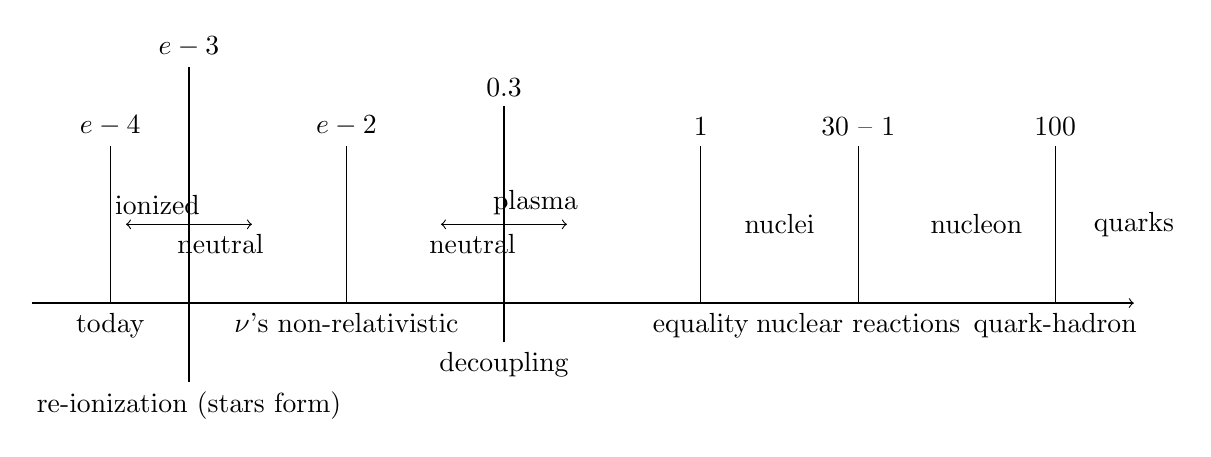
\begin{tikzpicture}
        \draw[->] (-7, 0) -- (7, 0);
        \draw (-6, 0) node[below]{today} -- (-6, 2) node[above]{$\SI{e-4}{\eV}$};
        \draw (-5, -1) node[below]{re-ionization (stars form)} -- (-5, 3) node[above]{$\SI{e-3}{\eV}$};
        \draw (-3, 0) node[below]{$\nu$'s non-relativistic} -- (-3, 2) node[above]{$\SI{e-2}{\eV}$};
        \draw (-1, -0.5) node[below]{decoupling} -- (-1, 2.5) node[above]{$\SI{0.3}{\eV}$};
        \draw (1.5, 0) node[below]{equality} -- (1.5, 2) node[above]{$\SI{1}{\eV}$};
        \draw (3.5, 0) node[below]{nuclear reactions} -- (3.5, 2) node[above]{$\SI{30}{\kilo\eV}$ -- $\SI{1}{\mega\eV}$};
        \draw (6, 0) node[below]{quark-hadron} -- (6, 2) node[above]{$\SI{100}{\mega\eV}$};
        \draw[|->] (-5, 1) -- node[above]{ionized} (-5.8, 1);
        \draw[|->] (-5, 1) -- node[below]{neutral} (-4.2, 1);
        \draw[|->] (-1, 1) -- node[above]{plasma} (-1+0.8, 1);
        \draw[|->] (-1, 1) -- node[below]{neutral} (-1-0.8, 1);
        \draw (2.5, 1) node{nuclei};
        \draw (5, 1) node{nucleon};
        \draw (7, 1) node{quarks};
    \end{tikzpicture}
\end{center}

In particle accelerators have reached energies on the order of $\sim\SI{}{\tera \eV}$. This represents the limit of known physics. We also suspect that quantum gravity becomes important on the Plank energy scales ($\SI{e21}{\mega \eV}$). The most massive particles we know of are the top quark ($\SI{180}{\giga \eV}$) and the Higgs boson ($\SI{125}{\giga \eV}$).

\subsection{Baryongenesis}
Why is it that almost everything around us is matter and not anti-matter. The Baryongenesis program aims to answer this question. We suspect that Baryongenesis occurs when $T \gtrsim \SI{e12}{\eV}$. Recall that the ratio of baryons to photons today is,
\[ \f{n_B}{n_\ga} = \SI{e-9}{} \]
Despite the abundance of photons, most of the energy is in matter today. It must be that in the early universe the number of baryons is slightly more than the number of anti-baryons.
\[ \f{n_B - n_{\bar B}}{n_B} \sim \SI{e-9}{} \]
All of the processes in the standard model conserve baryon number. This means that we should expect the \textit{exact} same number of baryons and anti-baryons. It is shocking that there remains a non-zero difference. The Sakharov conditions outline how this is possible,
\begin{enumerate}
    \item A Baryon number violating process
    \item Charge Conjugation (C) and Charge-Parity (CP) violating process
    \item Departure from thermal equilibrium
\end{enumerate}

Charge Conjugation indicates a process that occurs the exact same way if one exchanges all positive charges with negative charges. The Charge-Parity condition indicates a process that occurs the same way when all momentum and charges are flipped. Altogether, the Sakharov conditions suggest that we need to look for processes outside the standard model.

\section{Big Bang Nucleosynthesis}

The inception of big bang nucleosynthesis was due to a number of fields of physics including nuclear physics and relativity and the Manhattan project was a big influence. These sources led to the understanding (1930s - 1950s) of how stars are fueled and where heavy elements come from; i.e. from nuclear fusion in stars and supernovae.
\[ \text{H} \to \text{He}, \text{C}, \text{O}, \ldots \]
The principle component was the study of weak interactions and $\be$-decay.
\begin{align*}
    n &\rightarrow p^{+} + e^{-} + \bar \nu_e \\
    e^{+} + n &\leftrightarrow p^{+} + \bar \nu_e \\
    \nu_e + n &\leftrightarrow p^{+} + e^{-}
\end{align*}

One of the first papers on big bang nucleosynthesis was due to Alpher, Bethe, Gammow ($\al\be\ga$) in 1948 where they explained the origins of light elements like ${}^3$He, ${}^4$He, D, ${}^7$Li in which ${}^4$He made up about $25 \%$ of the mass with most produced in the big bang, some in stars.\\

The principles of helium formation are as follows:
\begin{enumerate}
    \item The mass of protons and neutrons differ,
    \[ m_p c^2 = \SI{938.3}{\mega \eV} \qquad m_p c^2 = \SI{939.6}{\mega \eV} \]
    \[ \br{m_n - m_p} c^2 \simeq \SI{1.3}{\mega \eV} \]
    \item Free neutrons (not bound to nucleus) decay at a rate $t_{1/2} \simeq \SI{620}{\s}$
    \item Bound neutrons can be stable.
\end{enumerate}
In the early universe (but when $n,p$'s are non-relativistic such that $E = \sqrt{m^2 c^4 + p^2 c^2} \approx m c^2 + \f{p^2}{2m}$) we have that the number density $n$ of neutrons $n$ and protons $p$ is,
\begin{align*}
    n
    &= \intl \f{\dif^3 p}{h^3} \f{1}{e^{E/kT} + 1} \\
    &= \intl \f{\dif^3 p}{h^3} e^{-E/kT} \qquad E \gg k T \\
    &= \intl \f{\dif^3 p}{h^3} e^{-mc^2/kT - p^2/2mkT} \\
    n &\propto e^{-mc^2/kT} \f{\br{mkT}^{3/2}}{h^3}
\end{align*}
Therefore the ratio for protons to neutrons is,
\[ \f{n_n}{n_p} = \br{\f{m_n}{m_p}}^{3/2} \exp\bs{- \f{\br{m_n - m_p}c^2}{k T}} \]
Therefore as temperatures $kT$ decrease, the ratio $\f{n_n}{n_p}$ goes down as well until we reach thermal equilibrium. This occurs at the decoupling of the weak interaction at $k T\tsb{dec} \simeq \SI{0.8}{\mega \eV}$. In essence, weak interactions are important for $T > T\tsb{dec}$ and not important for $T < T\tsb{dec}$ when $\f{n_n}{n_p}$ remains constant.
\[ \f{n_n}{n_p} \simeq \exp\br{-\f{\SI{1.3}{\mega\eV}}{\SI{0.8}{\mega\eV}}}\simeq \f{1}{5} \eq \label{eq:np}\]
However the production of light elements does not proceed exclusively forward until deuterium becomes stable (where not enough photons have energies greater that its binding energy of $\SI{2.2}{\mega \eV}$). This occurs around $kT \simeq \SI{0.06}{\eV}$ and where $t\tsb{nuc} \simeq \SI{340}{\s}$. During this time, any free neutrons will readily decay with half-life $t_{n,1/2}= \SI{610}{\s}$. Therefore up until the $t\tsb{nuc}$,the neutrons are decaying intro protons. Ignoring the change in proton number,
\[ \f{n_n}{n_p} \simeq \f{1}{5} \times \exp\br{- \f{t\tsb{nuc}\ln 2}{t_{n,1/2}}} \simeq \f{1}{7.3}  \]
How does this fix the helium-4 abundance? Approximate that the majority of produced elements is helium-4. This is somewhat valid in that it is the lightest stable nucleus (after the proton). Every helium-4 nucleus requires two neutrons. Therefore,
\[ n\tsb{He-4} = \f{n_n}{2}\]
But every helium-4 nucleus weighs roughly $4$ protons (neutrons). Therefore the mass fraction is,
\[ Y_4 = \f{4 (m_p + m_n)/2 n\tsb{He-4}}{m_n n_n + m_p + n_p} \]
Treating $m_p \simeq m_n$,
\[ Y_4 = \f{2 n_n}{n_n +n_p} = \f{2}{1 + n_p / n_n} \simeq 0.24 \]
Which agrees with the observed amount of $25 \%$.

\section{Cosmic Inflation}

Inflation was invented by a number of researchers:
\begin{itemize}
    \item Alan Guth (1981) $\to$ Old Inflation
    \item Alexei Starobinsky (1979)
    \item Andrei Linde (1981) $\to$ New Inflation
\end{itemize}

Inflation was invented to solve a number of problems with hot big bang cosmologies:
\begin{enumerate}
    \item \term{Flatness Problem}: Today we know that $\Om_k$ is small (very conservatively $0.5 \leq \Om\tsb{tot} \leq 1.5$),
    \[ \abs{\Om\tsb{tot}\br{t} - 1} = \f{\abs{k}}{a^2 H^2} \leq 1 \]
    If we consider the dynamics of $\Om_k$, $a^2 H^2 \propto t^{-1}$ in a radiation dominated era and $a^2 H^2 \propto t^{-2/3}$ in a matter dominated era. Therefore, $\Om_k$ \textbf{grows} over time. Since today $\Om_k$ is small, it had to be far smaller in the past:
    \[ \abs{\Om\tsb{tot} - 1} \simeq \underbrace{10^{-5}}_{\text{decoupling}}, \underbrace{10^{-18}}_{\text{BBN}}, \underbrace{10^{-30}}_{\text{electroweak}}, \underbrace{10^{-60}}_{\text{Planck}} \]
    This is an issue of \textit{fine-tuning}.
    \item \term{Horizon Problem}: In a flat, radiation dominated universe, $c \dif t = a \dif r$ therefore,
    \[ a = a\tsb{dec} \br{\f{t}{t}}^{} \]
\end{enumerate}

\subsection{Origin of Structure in the Universe}
\todo[TC]{Beginning of this lecture is weak}

Quantum fluctuations during inflation are on the order of,
\[  \f{\de T}{T} = \SI{e-5}{}\]
This means that,
\[ \f{H}{M_p} \sim \br{\f{k T\tsb{rad}}{M_p c^2}}^2 \implies k T\tsb{rad} = \SI{e15}{\giga\eV} \]
At the end of inflation the universe begins a phase of reheating. This means that $\La\tsb{inf}$ has to go away in order to begin a radiation dominated era. The $w$ parameter ($w = \f{p}{\rho c^2}$)
\begin{alignat*}{2}
    w &< -\f13 \quad &&\text{Inflation}\\
    w &\approx -1 \quad &&\text{Inflation can end}\\
    w &= -1 \quad &&\text{exact $\La$}
\end{alignat*}

\[ H = \br{8 \pi G}{3} \rho \]
\[ \dot \rho + 3 H \br{\rho + p c^2} = 0 \implies \f{\dif \ln \rho}{\dif \ln a} + 3 \br{1 + w} = 0 \]
Therefore,
\[ \rho \propto a^{- 3\br{1 + w}} \]
Since we know that $\rho + p c^2 > 0$, it must be that $w > -1$. This is known as the \textit{null energy condition}.
\[ \der{\ln a}{t} \propto a^{- \f{3\br{1 + w}}{2}} \]
Integrating gives,
\[ t \propto \int e^{\f32 \br{1 + w} \ln a} \dif \la a = \f{2}{3 \br{1 + w}} a^{\f{3\br{1 + w}}{2}} - t_{*} \]
This means that $a$ has time dependence,
\[ a \propto \br{t - t_{*}}^{\f{2}{3\br{1 + w}}} \]
This means that regardless of the content of the universe, there exists a time $t_{*}$ where the scale goes to $a = 0$. This is the time of the Big Bang singularity. There are a number of caveats or loopholes to this result. First of course, there is always the possibility of $w = -1$. As it turns out, this universe is unstable. Second, if we have $k = 0$ then the universe is not spherical. In this case intuition suggests that a materials in the universe come closer and closer together as $a \to 0$, there remains the possibility of everything passing through each other and $a < 0$. As it turns out, in the 70's Penrose and Hawking demonstrated some singularity theorems that rule out this loophole. \\

Recall that classical electromagnetism predicted that the an electron orbiting a proton would continue to emit radiation until it reached the proton emitting an infinite amount of energy. In some sense, this can be considered as a singularity as well. It was quantum mechanics that resolved this issue and it is a hope that quantum gravity will resolve some of the issues with the Big Bang singularity in much the same way. \\

\subsection{Big Bang and Black Holes}

Black holes are best understood in turns of \textit{Penrose diagrams}. A Penrose diagram is a space time diagram that is deformed in such a way that light travels at $45^{o}$ and infinite distances and times become finite. A black hole can be depicted as,

\begin{center}
    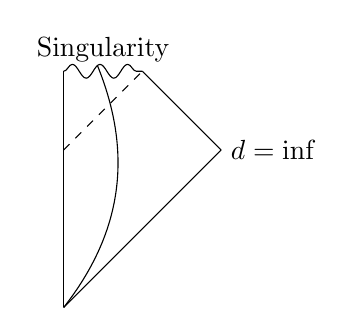
\begin{tikzpicture}
        \draw[]  (0,0) -- (0, 3);
        \draw[]  (0,0) -- (2, 2) node[right]{$d = \inf$};
        \draw[]  (2,2) -- (1, 3);
        \draw[decorate, decoration=snake] (0, 3) -- node[above]{Singularity} (1, 3);
        \draw[dashed]  (0,2) -- (1, 3);
        \path[] (0, 0) edge[bend right] (0.5 - 0.07, 3 + 0.07);
    \end{tikzpicture}
\end{center}

Another example is an eternal black hole,
\begin{center}
    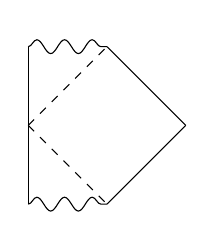
\begin{tikzpicture}
        \draw[]  (0,1) -- (0, 3);
        \draw[]  (1,1) -- (2, 2);
        \draw[]  (2,2) -- (1, 3);
        \draw[decorate, decoration=snake] (0, 3) -- node[above]{} (1, 3);
        \draw[decorate, decoration=snake] (0, 1) -- node[below]{} (1, 1);
        \draw[dashed]  (0,2) -- (1, 3);
        \draw[dashed]  (0,2) -- (1, 1);
    \end{tikzpicture}
\end{center}
\begin{center}
    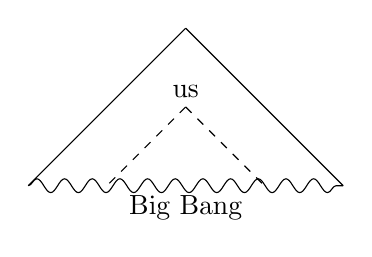
\begin{tikzpicture}
        \draw[]  (0,0) -- (-2, -2);
        \draw[]  (0,0) -- (2, -2);
        \draw[dashed]  (0, -1) node[above]{us} -- (1, -2);
        \draw[dashed]  (0, -1) -- (-1, -2);
        \draw[decorate, decoration=snake] (-2, -2) --node[below]{Big Bang} (2, -2);
    \end{tikzpicture}
\end{center}
\subsection{What's Wrong with Singularities}

A good enough analogy to singularities in spacetime is a classical electron around a proton. If the electron has frequency $\w$, we can approximate the acceleration of the electron,
\[ \f{e^2}{4 \pi \ep_0 r^2} = \f{m_e v^2}{r} = m_e \w^2 r \]
This means that the frequency scales with $r$,
\[ \w = \f{e}{\sqrt{4 \pi \ep_0 m_e } r^{3/2}} \]
The electron's electric field is then oscillating at the same frequency $\w$ which means that the emitted light has frequency $\w$. The energy of the electron is the potential energy due to the photon,
\[ E_e \sim \f{e^2}{4 \pi \ep_0 r} \]
This means that the energy lost has to go into the number of photons that are emitted,
\[ \# \text{Photons} = \f{e^2}{4 \pi \ep_0 r \hbar \w} \propto r^{1/2} \]
This means that at some point the number of photons emitted becomes fractional. However photons are quantized. Therefore we can roughly assume that the ground state of the hydrogen atom occurs when $\# \text{Photons} \sim 1$. \\

It is also possible to perform a similar analysis to the entire universe. What is the number of photons per horizon or Hubble radius. The reduced Planck mass is,
\[ M_p c^2 = E_p = \sqrt{\f{\hbar c}{8 \pi G}} = \SI{e18}{\giga \eV} \]
The number density of photons is roughly $T^3$ times the contained volume. With natural units,
\[ N \sim T^3 \times \f{1}{H^3} \]
But from the Friedmann equation $H^2 \sim T^4 / M_p^2$. Therefore,
\[ N \sim T^3 \times \f{M_p^3}{T^6} \sim \br{\f{M_p c^2}{k T}}^3 \]
This means that classical physics breaks down when $N \sim 1$ or when,
\[ kT \geq M_p c^2 \sim \SI{e18}{\giga \eV} \]

\subsection{Quantum Gravity}

What is Quantum Gravity? Quantum gravity is just an idea or collection of many ideas and not a theory like general relativity or quantum mechanics is. In order to solve or figure out quantum gravity, we need to determine what are the right ingredients or degrees of freedom. \\

The most popular theory of quantum gravity is string theory. The principle component being the idea that particles are not fundamental but are instead everything is made out of fundamental strings. The appeal or advantage of string theory is that fundamental strings can be quantized. However, string theory requires an additional $6$ extra dimensions. This makes the total number of dimensions $3 + 6 + 1 = 10$. This can be considered a failed prediction of string theory, although there is active research trying to hide these extra dimensions.\\

Alternatively, we can adopt the approach of discretizing space. Some attempts include loop quantum gravity or dynamical triangulation. \\

Additionally one can attempt to discretize \textit{spacetime} which forms causal sets. \\

Another possibility is \textit{emergent gravity}. This idea considers the possibility that Lorentz invariance is not fundamental and that at high enough energies, Lorentz symmetry breaks down. This allows for the possibility of superluminal propagations or information.

\subsection{Big Bang in Quantum Gravity}

There are a number of possibilities for the fate or nature of a ``Big Bang'' under the different theories of quantum gravity. Some of these include:
\begin{enumerate}
    \item Big Bounce: the contraction of space bounces off the singularity
    \item Quantum Geometry
    \item Big Bang is the start of time itself
\end{enumerate}

\todo[TC]{Missed a Lecture}

\section{Precision Cosmology}

\subsection{Six Parameters}
An important question to ask is: \textit{If we have a model that we believe is correct, how can we test it and assign a confidence to it?}\\

In the early stages of cosmology, there were a number of uncertainties within the observed data and disagreements between cosmologists. However recently, the later decades of cosmology have been marked by a heightened degree of precision and maturity. \\

To summarize what we have discussed so far, there are in practice $6$ parameters that characterize the simplest cosmological models. This is sometimes referred to as \textit{vanilla} $\La$CDM. These values are referenced from \url{https://arxiv.org/pdf/1502.01589v3.pdf}.
\begin{center}
\begin{tabular}{|c|c|c|c|}
    \hline
    Number & Parameter & Value & Source \\
    \hline
    1 & Hubble $h$ & $\SI{0.673\pm0.012}{}$ & expansion, $3\si$ with supernovae \\
    2 & Dark Matter $\Om\tsb{dm}h^2$ & $\SI{0.1198\pm0.0026}{}$ & CDM density \\
    3 & Baryons $\Om\tsb{b}h^2$ & $\SI{0.02207\pm0.00027}{}$ & Baryon density \\
    4 & Tilt $n_s$ & $\SI{0.965\pm0.005}{}$ &  \\
    5 & Amplitude $\De_0^2$ & ${\SI{2.143\pm0.052}{}} \times \SI{e-9}{}$ &  \\
    6 & Optical Depth to Re-ionization $\tau$ & ${\SI{0.078\pm0.019}{}}$ &  \\
    \hline
\end{tabular}
\end{center}

Where $n_s$ and $\De_0^2$ are fluctuation parameters associated with the primordial density fluctuations of baryons,
\[ \ba{\br{\f{\de \rho}{\rho}}^2}\tsb{primordial}\br{r} \approx \De_0^2 \br{\f{r}{\SI{20}{\mega\pc}}}^{1-n_s} \]
Notice that if $n_s = 1$, then there would be the same structure at all radial scales. \\

The final parameter $\tau$ is the optical depth to re-ionization and can in principle be deduced from the previous $5$ parameters. However, a measurement depends on astrophysical phenomena. Recall that the last scattering surface (LSS) is at a farther distance than the re-ionization surface. As photons travel from LSS towards us, they are scattered by ionized material within the RIS.

\begin{center}
    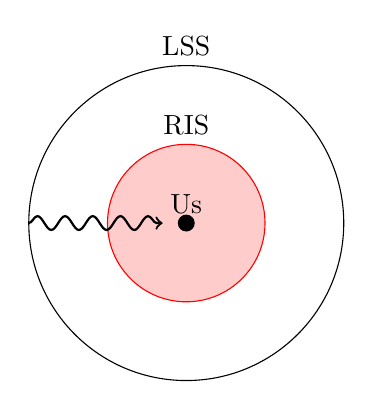
\begin{tikzpicture}
        \draw[red, fill, fill opacity=0.2] (0,0) circle (1);
        \draw (0,0) circle (2);
        \draw (0, 2) node[above]{LSS};
        \draw (0, 1) node[above]{RIS};
        \draw[fill] (0,0) circle (0.1) node[above]{Us};
        \draw[thick, ->, decorate, decoration=snake] (-2, 0) -- (-0.3,0);
    \end{tikzpicture}
\end{center}

The remainder of cosmological parameters can we calculated from the above $6$ via simple or complicated equations. For example,
\begin{align*}
    \text{Age} &\simeq \SI{13.8}{\giga\yr} \\
    D\tsb{LSS} &\simeq \SI{14}{\giga\pc} \\
    \Om_{\La} &\simeq \SI{0.69}{} \\
    \Om_{m} &\simeq \SI{0.31}{}
\end{align*}

\subsection{Auxiliary Parameters}
There are also a number of auxiliary parameters that can be measured directly and are currently in agreement with a vanilla $\La$CDM. For example spatial curvature is nearly zero.
\[ \abs{\Om_{k}} \lesssim \SI{0.005}{} \]
There are also parameters associated with neutrino. First the total neutrino masses are constrained by neutrino oscillations and other observations,
\[ \SI{0.05}{\eV} < \sum {m_{\nu}} < \SI{0.2}{\eV} \]
The effective number density is also an auxiliary parameter,
\[ N\tsb{eff} = \SI{3.04\pm0.33}{} \]
Moreover the Helium abundance can be measured directly but can be calculated with consistency from BBN,
\[ Y_4 \simeq \SI{0.249\pm0.025}{} \]
Another parameter is the contribution of gravity waves from the Big Bang. These gravitational waves are at much longer wavelengths than those measured by LIGO. In principle these waves could be measured but no direct measurements have currently been made.
\[ r < 0.113 \]
It turns out that some inflation models predict Big Bang gravitational waves.\\

Another auxiliary parameter is the $w$ dark energy equation of state $w = - P / \rho c^2$
\[ w = - \SI{1.02\pm0.008}{} \]
Recall that our models predict a cosmological constant $w = -1$ but one could assume this parameter is not fixed and measure it directly. \\

Precision cosmology current only requires the main $6$ parameters and the remainder can be calculated. However, more precise models might require the addition of some of these extra parameters.

\subsection{Data}

The CMB anisotropies are the most important data set we have for constraining the $6$ parameters of a vanilla $\La$CMB. This is due to the following facts:
\begin{enumerate}
    \item Relatively easy to observe
    \item Clean source
    \item Governed by linear equations
\end{enumerate}
In terms of the CMB we talked a lot about temperature $T$ and their anisotropies. In addition to temperatures, we can also measure the polarization of of the photons coming from the CMB. Furthermore, it is possible to measure the affects of gravitational lensing due to the materials and energy between us and the surface of last scattering.\\

The CMB, however, does not completely determine all cosmological parameters. The CMB is not entirely sensitive to certain parameters. As a result, other observations are necessary to compliment the CMB. A number of Galaxy surveys have accomplished this. \\

As an example, Baryonic Acoustic Oscillations (BAO) are used as a standard ruler to measure the tomography of the universe. Additionally, measurements of supernovae (specifically type $1a$), Hubble measurements and the counting of galaxy clusters embellish the CMB nicely. Nonetheless, these later methods are based on non-linear dynamics and less understand and thus more contested.

\subsection{Statistics}

Statistics are the primal component of assigning confidence to physical models. \term{Bayesian Analysis} is useful in nearly all fields of scientific analysis. Bayes theorem determines a relationship between conditional probabilities.

\begin{center}
    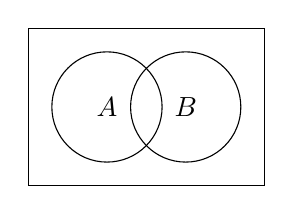
\begin{tikzpicture}
        \draw[] (0,0) -- (0,2) -- (3,2) -- (3,0) -- cycle;
        \draw (1,1) circle (0.7);
        \draw (1,1) node[]{$A$};
        \draw (2,1) circle (0.7);
        \draw (2,1) node[]{$B$};
    \end{tikzpicture}
\end{center}

Bayes theorem says,
\[ P\br{A \mid B} = \f{P\br{A,B}}{P\br{B}} \]
And as a corollary,
\[ P\br{A \mid B} P\br{B} = P\br{B \mid A}P\br{A} \]
When applied to physical models,
\[ P\br{\text{params}\mid\text{data}}\propto P\br{\text{data}\mid\text{params}}P\br{\text{params}} \]
Where we refer to different components of this equation with special names,
\begin{center}
    \begin{tabular}{cc}
        posterior & $P\br{\text{params}\mid\text{data}}$ \\
        likelihood & $P\br{\text{data}\mid\text{params}}$ \\
        prior & $P\br{\text{params}}$ \\
    \end{tabular}
\end{center}

The most common model for likelihood estimation is a Gaussian model,
\[ P\br{\text{data}\mid\text{params}} \propto \exp\br{-\f12 \sum_i \f{\bs{D_i - M_i\br{p}}}{\si_i^2}} \]
Where $\si_i^2$ is the error in the data/model and $D_i$ is the observed data and $M_i\br{p}$ is the model-predicted value associated with measured data $D_i$. In order to maximize the likelihood, one simply varies the parameters $p$ in order to match the data. The set of parameters $p$ can be any size (and is $6$ in the case of precision cosmology). To visualize the process, consider the parameter space determined by $\Om_b h^2$ and $\Om_m h^2$.
\begin{center}
    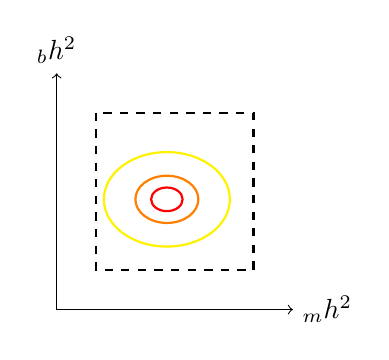
\begin{tikzpicture}
        \pgfmathsetmacro{\pad}{0.5}
        \draw[<->] (0,3) node[above]{$\Om_b h^2$} -- (0, 0) -- (3, 0) node[right]{$\Om_m h^2$};
        \draw[dashed, thick] (0 + \pad, 3 - \pad) -- (0 + \pad,0 + \pad) -- (3 - \pad, 0 + \pad) -- (3 - \pad,3 - \pad) -- cycle;
        \draw[thick, red] (1.4,1.4) ellipse (0.2 and 0.15);
        \draw[thick, orange] (1.4,1.4) ellipse (0.4 and 0.3);
        \draw[thick, yellow] (1.4,1.4) ellipse (0.8 and 0.6);
    \end{tikzpicture}
\end{center}
First one normalizes the parameter space $\int P\dif p = 1$ and then determine $\si$ ranges,
\begin{align*}
    \int\tsb{region} P\br{p \mid D} \dif p
    &\simeq 68\% \quad 1\si \text{ region} \\
    &\simeq 95\% \quad 2\si \text{ region} \\
    &\simeq 99\% \quad 3\si \text{ region} \\
\end{align*}
A \textit{good} model with $N$ data points subtract the number of parameters, the $\chi^2$ value is,
\[ \chi^2 \simeq N \pm \sqrt{2N} \]
Then the reduced $\chi^2$ value is,
\[ \chi\tsb{red}^2 \simeq 1 \pm \sqrt{\f2N} \]

\newpage
\section*{Appendix}
\markboth{Appendix}{Appendix}
\addcontentsline{toc}{section}{Appendix}
\setcounter{subsection}{0}
\setcounter{subsubsection}{0}
\renewcommand*{\theHsubsection}{appendix.\the\value{subsection}}
\renewcommand{\thesubsection}{\Alph{subsection}}
\subsection{High Frequency Blackbody Spectrum}
\label{sec:upper_black_body}

First begin by calculating the number density for photons as predicted by a Blackbody spectrum. The energy per unit volume per unit time per frequency is given by,
\[ \f{\dif E}{\dif V \dif f} = \ep_f = \f{8 \pi h f^3}{c^3 \bs{e^{h f/ k T} - 1}}\]
Thus the number density of photons between $f$ and $f + \dif f$ is given by,
\[ n_f = \f{\ep_f \dif f}{h f}  = \f{8 \pi f^2}{c^3 \bs{e^{h f/ k T} - 1}} \dif f\]
Therefore the total number density can be calculate by integrating over all frequencies,
\[ n = \intl_{0}^{\inf} n_f = \intl_{0}^{\inf} \f{8 \pi f^2}{c^3 \bs{e^{h f/ k T} - 1}} \dif f\]
Simplifying,
\[ n = \f{8 \pi}{c^3}\br{\f{kT}{h}}^3 \intl_{0}^{\inf} \f{ x^2}{{e^{x} - 1}} \dif x\]
Recall the relationship between the Riemann Zeta function and the Gamma function\footnote{\url{http://mathworld.wolfram.com/GammaFunction.html}},
\[ \zeta\br{z}\Ga\br{z} = \intl_{0}^{\inf} \f{x^{z-1}}{e^{x} - 1}\dif x \]
Therefore,
\[ n = 16 \pi \zeta\br{3} \br{\f{k T}{hc}}^3 \]
However, we are interested in the number density with energy (and thus frequency) greater than some threshold. Let this energy/frequency uppper limit be $E^* = h f^*$ such that,
\[ n_{> f^*} = \intl_{f^{*}}^{\inf} \f{8 \pi f^2}{c^3 \bs{e^{h f/ k T} - 1}} \dif f = \f{8 \pi}{c^3}\br{\f{kT}{h}}^3 \intl_{x^*}^{\inf} \f{ x^2}{{e^{x} - 1}} \dif x \]
Where $x^*$ is equal to $h f^{*} / k T$. We further make the assumption that,
\[ h f^{*} \gg k T \]
i.e. it is far colder than the ionization energy scale and that only the tail end of the spectrum will contribute. Therefore $x^* \gg 1$. Therefore,
\[ \intl_{x^*}^{\inf} \f{ x^2}{{e^{x} - 1}} \dif x \simeq \intl_{x^*}^{\inf} \f{ x^2}{e^{x}} \dif x = \intl_{x^*}^{\inf} x^2 e^{-x} \dif x \]
This later integral can be easily calculated,
\begin{align*}
\intl_{a}^{b} x^2 e^{\al x} \dif x
&= \intl_{a}^{b} \der{}{\al} x e^{\al x} \dif x \\
&= \intl_{a}^{b} \dder{}{\al}e^{\al x} \dif x \\
&= \dder{}{\al} \intl_{a}^{b} e^{\al x} \dif x \\
&= \dder{}{\al} \f{1}{\al}\br{e^{\al b} - e^{\al a}} \\
&= \der{}{\al} \f{\br{b e^{\al b} - a e^{\al}}\al - \br{e^{\al b} - e^{\al}}}{\al^2} \\
&= \f{e^{\al b} \br{b \al \br{b \al - 2} + 2} - e^{\al a} \br{a \al \br{a \al - 2} + 2}}{\al^3}
\end{align*}
Then set $\al = -1$, $a = x^{*}, b= \inf$,
\[ \intl_{x^*}^{\inf} x^2 e^{-x} \dif x = e^{- x^{*}} \br{-x^{*} \br{- x^{*} - 2} + 2} \]
Again make use of the approximation that $x^{*} \gg 1$,
\[ \intl_{x^*}^{\inf} x^2 e^{-x} \dif x \simeq e^{- x^{*}} \br{x^{*}}^2 \]
Which could have been approximated just by exposing the integrand by setting $x = x^*$. Nonetheless, we now have the approximation,
\[ n_{> f^*} \simeq \f{8 \pi}{c^3}\br{\f{kT}{h}}^3 e^{- h f^{*}/ kT} \br{\f{h f^{*}}{kT}}^2 \]
We also have the ratio,
\[ \f{n_{> f^*}}{n} \simeq \f{1}{2 \zeta\br{3}}e^{- h f^{*}/ kT} \br{\f{h f^{*}}{kT}}^2 \]

\subsection{Dominating Eras}

\begin{center}
\begin{tabular}{|c|c|c|c|c|}
    \hline
     & Matter & Radiation & Cosmological Constant & Curvature \\
    \hline
    $w$ & $0$ & $\f13$ & $-1$ & $-\f13$ \\
    \hline
    $\rho\br{a} \propto a^{-3\br{1 + w}}$ & $a^{-3}$ & $a^{-4}$ & $1$ & $a^{-2}$ \\
    \hline
    $a\br{t} \propto t^{\f23\br{\f{1}{1 + w}}}$ & $t^{2/3}$ & $t^{1/2}$ & $\exp\br{\sqrt{\f{\La}{t}} t}$ & $t$ \\
    \hline
    $\rho\br{t} \propto t^{-2}$ & $t^{-2}$ & $t^{-2}$ & $1$ & $t^{-2}$ \\
    \hline
\end{tabular}
\end{center}

Equation of State:
\[ p = w\rho c^2 \]
Fluid Equation governs $\rho\br{t}$:
\[ \dot \rho + 3 \f{\dot a}{a} \br{\rho + \f{p}{c^2}} = 0 \]
For $w$-dominant era:
\[ \dot \rho + 3 \f{\dot a}{a} \br{1 + w}\rho = 0 \]
\[ a \dot \rho + 3\br{1 + w} \dot a \rho = 0 \]
\[ \f{1}{a^{3\br{1 + w} - 1}} \der{}{t}\br{\rho a^{3\br{1 + w}}} = 0 \]
\[ \der{}{t}\br{\rho a^{3\br{1 + w}}} = 0 \]
\[ \rho a^{3\br{1 + w}} = \text{const.} \]
\[ \rho \propto a^{-3\br{1 + w}} \]
The most general Friedmann equation:
\[ H^2 \br{a} = \br{\f{\dot a}{a}}^2 = \f{8 \pi G}{3} \br{\rho_m + \rho_r} + \f{\La}{3} - \f{k}{a^2} = \f{8 \pi G}{3} \br{\rho_m + \rho_r + \rho_\La + \rho_k} \]
\[ \rho_k = - \f{3}{8 \pi G} a^2 \]
\[ \rho_\La = \f{\La}{8 \pi G} \]
For a dominant density,
\[ \br{\f{\dot a}{a}}^2 = \f{8 \pi G}{3} \rho \propto a^{-3\br{1 + w}} \]
\[ \dot a^2 \propto a^{-3\br{1 + w} +2} \]
\[ \dot a \propto a^{-\f32\br{1 + w} + 1} \]
\[ a^{\f32\br{1 + w} - 1} \dif a \propto \dif t  \]
For $w \neq -1$,
\[ a^{\f32\br{1 + w}} \propto t  \]
\[ a \propto t^{\f23\br{\f{1}{1 + w}}}  \]
\[ \rho \propto \br{t^{\f23\br{\f{1}{1 + w}}}}^{-3\br{1 + w}} \propto t^{-2} \]
For $w = -1$,
\[ \br{\f{\dot a}{a}}^2 \propto \f{\La}{3}  \]
\[ a = \exp\br{\sqrt{\f{\La}{t}} t} \]


\end{document}